\chapter[Inestabilidades en un OBHL]{Radiaci\'{o}n de Hawking an\'{a}loga como una inestabilidad en un OBHL}\label{cap5}

La propagaci\'{o}n de la luz en medios no lineales como las fibras \'{o}pticas permite la existencia de solitones, i.e., pulsos de luz cuyo perfil de intensidad no cambia a lo largo del medio donde se propagan. La no linealidad del material permite la interacción entre estos pulsos y un paquete de ondas de menor intensidad (pulso de prueba) permitiendo as\'{i} construir un análogo de horizonte de eventos, similar a los existentes en el contexto de gravitaci\'{o}n.\\

Una predicción notable que surgió del estudio de los an\'{a}logos de gravedad  es que la combinación de un  horizonte de agujero negro junto a un horizonte de agujero blanco lleva a un proceso de amplificación de la radiaci\'{o}n que se encuentra entre ellos, muy similar a un láser, en donde la radiación rebota cont\'{i}nuamente entre la cavidad teniendo como resultado la amplificaci\'{o}n del campo.\\

El láser de agujeros negros (BHL) se propuso inicialmente para sistemas que exhiben una dispersión superlum\'{i}nica o an\'{o}mala, en los que la velocidad de grupo aumenta con la frecuencia, relaci\'{o}n que cumplen los an\'{a}logos ac\'{u}sticos como los condensados de Bose-Einstein (BECs) \citep{Corley1999}. En estos sistemas, la cavidad donde el campo bos\'{o}nico se amplifica se construye a partir de un cambio en la velocidad del fluido. Para llevar estas ideas al caso \'{o}ptico, se requiere una relaci\'{o}n de dispersi\'{o}n normal \citep{GaonaReyes2017} y construir una cavidad no con un medio en movimiento, si no mediante las propiedades mismas que siguen las ondas al propagarse por el medio.\\

La radiaci\'{o}n confinada en la cavidad formada por los dos horizontes de BH y WH son modos resonantes que en cada reflexi\'on con la cavidad aumentan su amplitud para conservar la frecuencia com\'{o}vil y la norma en su evoluci\'{o}n \citep{Robertson2011}. Este comportamiento se puede analizar a partir de teor\'{i}a de inestabilidades.\\

Como se present\'{o} en la secci\'{o}n \ref{sec:Inestabilidad} y el cap\'{i}tulo \ref{cap3}, las inestabilidades son inherentes en el an\'{a}lisis de la din\'{a}mica una fluctuaci\'{o}n generada en un fluido con movimiento \citep{Hydrodynamic}. Hemos descrito el campo o fluctuaci\'{o}n que se genera en un medio con movimiento a partir de los modos normales en que \'{e}ste oscila. Estos modos son ondas planas de la forma $\exp[-i(\omega \tau+\omega' \zeta)]$, donde $\omega$ denota la frecuencia del modo en el marco de laboratorio y $\omega'$ la frecuencia en el marco com\'{o}vil. Usualmente estas frecuencias toman valores reales cuando describen una onda, pero en el vocabulario de inestabilidades hidrodinámicas, estas ondas se denominan\textit{ ondas neutrales} y pueden ser generalizadas permitiendo que $\omega$ y $\omega'$ sean cantidades complejas con el fin de predecir los procesos de amplificaci\'{o}n de una fluctuaci\'{o}n cuando se propaga en un fluido en movimiento.\\

En el caso de $\omega \in \mathbb{R}$  y $\omega'=\omega'_R+i\omega'_I \in \mathbb{C}$ se tiene una \textit{inestabilidad temporal} y corresponde a la situación física donde se impone un forzamiento al flujo (en nuestro caso es tener un perfil de velocidades para el medio). Si hay una frecuencia para el cual $\omega'_I(\omega)>0$  entonces la perturbación crece exponencialmente y el flujo se considera linealmente inestable. Un modo con $\omega'_I=0$ se llama \textit{neutral}, que es el caso t\'{i}pico, mientras que un modo con $\omega'_I<0$ se conoce como\textit{ amortiguado} o\textit{ estable} \citep{gallaire2017fluid}. Los modos neutrales se han usado para describir la amplificaci\'{o}n de un campo $\phi$ y encontrar las frecuencias $\omega'$ en que se obtienen resonancias en la configuraci\'{o}n de un l\'{a}ser \'{o}ptico de agujeros negros (OBHL) \citep{Faccio2012} y \citep{GaonaReyes2017}. Pero, ¿es posible predecir estos mismos resultados describiendo los modos en que oscila $\phi$ como inestabilidades temporales? En este cap\'{i}tulo se dar\'{a} respuesta a esta pregunta. Para ello se iniciar\'{a} considerando el modelo simple para un OBHL, se analiza la relaci\'{o}n de dispersi\'{o}n de forma cl\'{a}sica, i.e., usando el m\'{e}todo gr\'{a}fico donde solo se permite que $\omega$ y $\omega'$ sean reales, luego se generaliza el problema permitiendo que las frecuencias en el marco de laboratorio y com\'{o}vil sean complejas, teniendo como requerimiento que el campo que describe los modos de la cavidad sea de cuadrado integrable.\\

Por \'{u}ltimo, se comparan los resultados obtenidos del problema generalizado con los que se esperan por un  m\'{e}todo simple, verificando que la radiaci\'{o}n resonante en la cavidad puede ser vista como el producto de una inestabilidad temporal. Con el modelo de inestabilidades no solo se reproducen los resultados ya conocidos, sino que adem\'{a}s  nos permite predecir un nuevo comportamiento del campo que no se obtiene con el modelo simple, como es que la radiaci\'{o}n atrapada entre los horizontes que forman la cavidad puede tunelar y escapar de ella, similar al comportamiento habitual  de la radiaci\'{o}n de Hawking. Solo para condiciones muy espec\'{i}ficas se pueden obtener modos para los cuales hay una mayor probabilidad de encontrar el campo dentro de la cavidad que fuera de ella. Este \'{u}ltimo  resultado est\'{a} de acuerdo con los monomodos que se propagan en una gu\'{i}a de onda temporal expuesta en \cite{Plansinis2016}.
\section{M\'{e}todo gr\'{a}fico: OBHL con frecuencias reales}\label{realo}

La idea básica de un OBHL es atrapar un pulso de prueba que ser\'{a} una fluctuaci\'{o}n del vac\'{i}o  en una cavidad formada por dos solitones separados una distancia $L_c$ (o tiempo $\tau_c$) dentro de la fibra. En el contexto de \'{o}ptica no lineal esta configuraci\'{o}n es conocida como gu\'{i}a de ondas temporal \citep{Plansinis2016}.\\

La configuraci\'{o}n del OBHL solo existe para ciertos valores de $\omega'$, aquellos que quedan delimitados por los valores m\'{a}ximos de las relaciones de dispersi\'{o}n definidas en la regi\'{o}n lenta con $\delta n=\delta n_{\text{max}}$ y la regi\'{o}n r\'{a}pida con $\delta n=0$, es decir, el rango de frecuencias en el marco com\'{o}vil est\'{a} dado por $(\omega'(\omega_{\text{h-max}}),\omega'(\omega_{\text{h}}))$, donde $\omega_{\text{h-max}}$, $\omega_{\text{h}}$ son frecuencias en el marco de laboratorio. En la figura \ref{fig:5.0} se muestra la relaci\'{o}n de dispersi\'{o}n ec. (\ref{ec:dispersion}) para frecuencias positivas donde es v\'{a}lida la configuraci\'{o}n del OBHL. \\

Iniciemos recordando que la relaci\'{o}n de dispersi\'{o}n que debe cumplir una fluctuaci\'{o}n en el interior de la fibra \'{o}ptica es
\begin{align}\label{ec:dispersion}
(\omega'-\upsilon (\tau)\omega)^2=\omega^2+\frac{\omega^4}{\Omega_0^2},
\end{align}
donde $\upsilon(\tau)=-n_{g0}+\delta n$ indica el \'{i}ndice de refracci\'{o}n efectivo que sienten los modos al moverse en la configuraci\'{o}n del OBHL. Esta cantidad ser\'{a} una velocidad adimensional negativa e indica la \textit{ velocidad} con la que se mueve la fibra \'{o}ptica (recuerde que en el an\'{a}logo \'{o}ptico el medio en movimiento se consigue por medio de las propiedades no lineales del material y no modificando la velocidad del medio).\\





\begin{figure}\centering
	\includegraphics[scale=0.5]{F51}
	\caption{Relaci\'{o}n de dispersi\'{o}n en el marco com\'{o}vil para frecuencias positivas. La franja rosa indica el intervalo en frecuencias del marco com\'{o}vil donde es permitida la configuraci\'{o}n del OBHL, la curva morada indica la relaci\'{o}n de dispersi\'{o}n que siguen los modos que se mueven en la regi\'{o}n lenta $\delta n=\delta n_{\text{max}}=0.1$ en la ec. (\ref{ec:dispersion}) y la curva verde es la relaci\'{o}n de dispersi\'{o}n para los modos en la regi\'{o}n r\'{a}pida, donde $\delta n=0.$}\label{fig:5.0}
\end{figure}

Si en el interior de la cavidad se genera de forma espont\'{a}nea una fluctuaci\'{o}n del vac\'{i}o con frecuencia $\omega_{\text{2ul}}$, su frecuencia en el marco com\'{o}vil $\omega'(\omega_{\text{2ul}})$ se conserva, por tanto puede dispersarse en cuatro modos posibles  en el interior de la cavidad y dos m\'{a}s en el exterior de ella. Estos modos se muestran en la figura \ref{fig:5.1}(a) y son las posibles soluciones de la relaci\'{o}n de dispersi\'{o}n de la ec. (\ref{ec:dispersion}) por el m\'{e}todo gr\'{a}fico cuando la velocidad $\upsilon(\tau)$ toma dos posibles valores: $\upsilon_1=-n_{g0}+\delta n_{\text{max}}$ y $\upsilon_2=-n_{g0}$, donde $\upsilon_1$ es el perfil que sienten las fluctuacion en las regiones $\text{I}$ y $\text{III}$ fuera de la cavidad, mientras que  $\upsilon_2$    es el  \'{i}ndice de grupo en el interior de la cavidad o regi\'{o}n $\text{II}$.\\

De igual modo que en el sistema ac\'{u}stico trabajado en el cap\'{i}tulo \ref{cap3}, $\upsilon_1$ define la regi\'{o}n \textit{lenta}, y es la zona donde la velocidad de las fluctuaciones es menor que la velocidad con la que fluye el medio, mientras que $\upsilon_2$ representa la regi\'{o}n \textit{r\'{a}pida} y es donde las fluctuaciones se mueven sin ver un \'{i}ndice de refraci\'{o}n extra, i.e., solo sienten el \'{i}ndice de grupo de la fibra $n_{g0}$. Esto hace que en el caso \'{o}ptico solo sea posible variar $\upsilon_1$ y $\upsilon_2$ se mantiene fijo.\\

Los modos $\omega$ que son soluci\'{o}n a la ec. (\ref{ec:dispersion}) est\'{a}n etiquetados por los sub\'{i}ndices 'u' o 'v', que indican si el modo est\'{a} en la rama contrapropagante o copropagante respectivamente. En la figura \ref{fig:5.1}(a), la rama copropagante para el rango de frecuencias $\omega'$ en que funciona el OBHL es una l\'{i}nea recta, indicando que estos modos no sufren dispersi\'{o}n cuando se propagan en el material, mientras que la rama contrapropagante es la l\'{i}nea curva que indica que los efectos dispersivos alteran m\'{a}s a estos modos. Con $\omega<0$, existen para $\upsilon_1$ y $\upsilon_2$ soluciones etiquetadas $\omega_{\text{1u}}$ y $\omega_{\text{2u}}$ y representan los modos de frecuencia y norma negativas definidos al final de la secci\'{o}n \ref{normaneg}. Para $\omega>0$ y  $\upsilon_1$ solo es encuentra una soluci\'{o}n en la rama copropagante $\omega_{\text{1v}}$, mientras que para $\upsilon_2$ existen tres modos, uno copropagante $\omega_{\text{2v}}$ y dos contrapropagantes $\omega_{\text{2ul}}$ y $\omega_{\text{2ur}}$, el sub\'{i}ndice (l) y (r) en estas dos \'{u}ltimas soluciones indican que los modos se mueven a la izquierda y derecha en el marco com\'{o}vil, respectivamente.\\

Ahora la configuraci\'{o}n de OBHL se logra cuando el flujo de velocidad creado por el cambio del \'{i}ndice de refraci\'{o}n var\'{i}a de una regi\'{o}n lenta $\upsilon_1$ (regi\'{o}n I) a un regi\'{o}n r\'{a}pida  $\upsilon_2$ (regi\'{o}n II) en un rango finito $\tau_c$ y regresa de nuevo a una velocidad $\upsilon_1$ (regi\'{o}n III), lo cual se logra con el perfil de velocidades dado en la figura \ref{fig:5.1}(b). La regi\'{o}n $\text{II}$ representa el interior de la cavidad. En ella los modos que son soluci\'{o}n a la relaci\'{o}n de dispersi\'{o}n se amplificar\'{a}n. En part\'{i}cular, los modos $\omega_{\text{2ul}}$ y $\omega_{\text{2ur}}$ cumplen una condici\'{o}n de resonancia que permite obtener estados confinados en la cavidad.
\begin{figure}
   \centering
   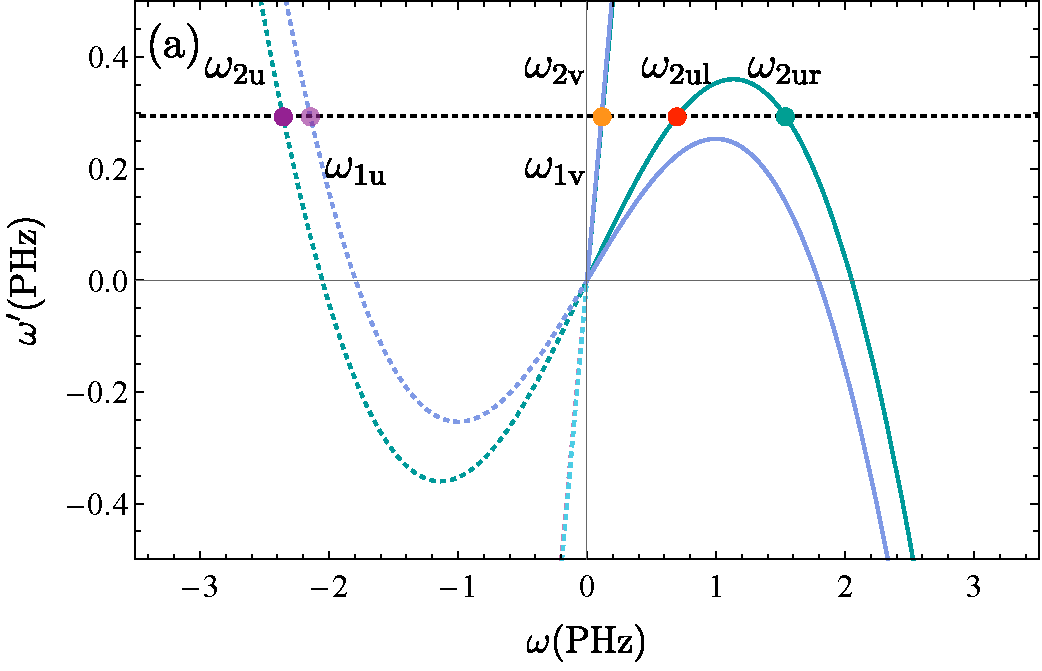
\includegraphics[height=5cm]{f52a.pdf}%
   \hspace{0.1cm}% add some horizontal spacing
   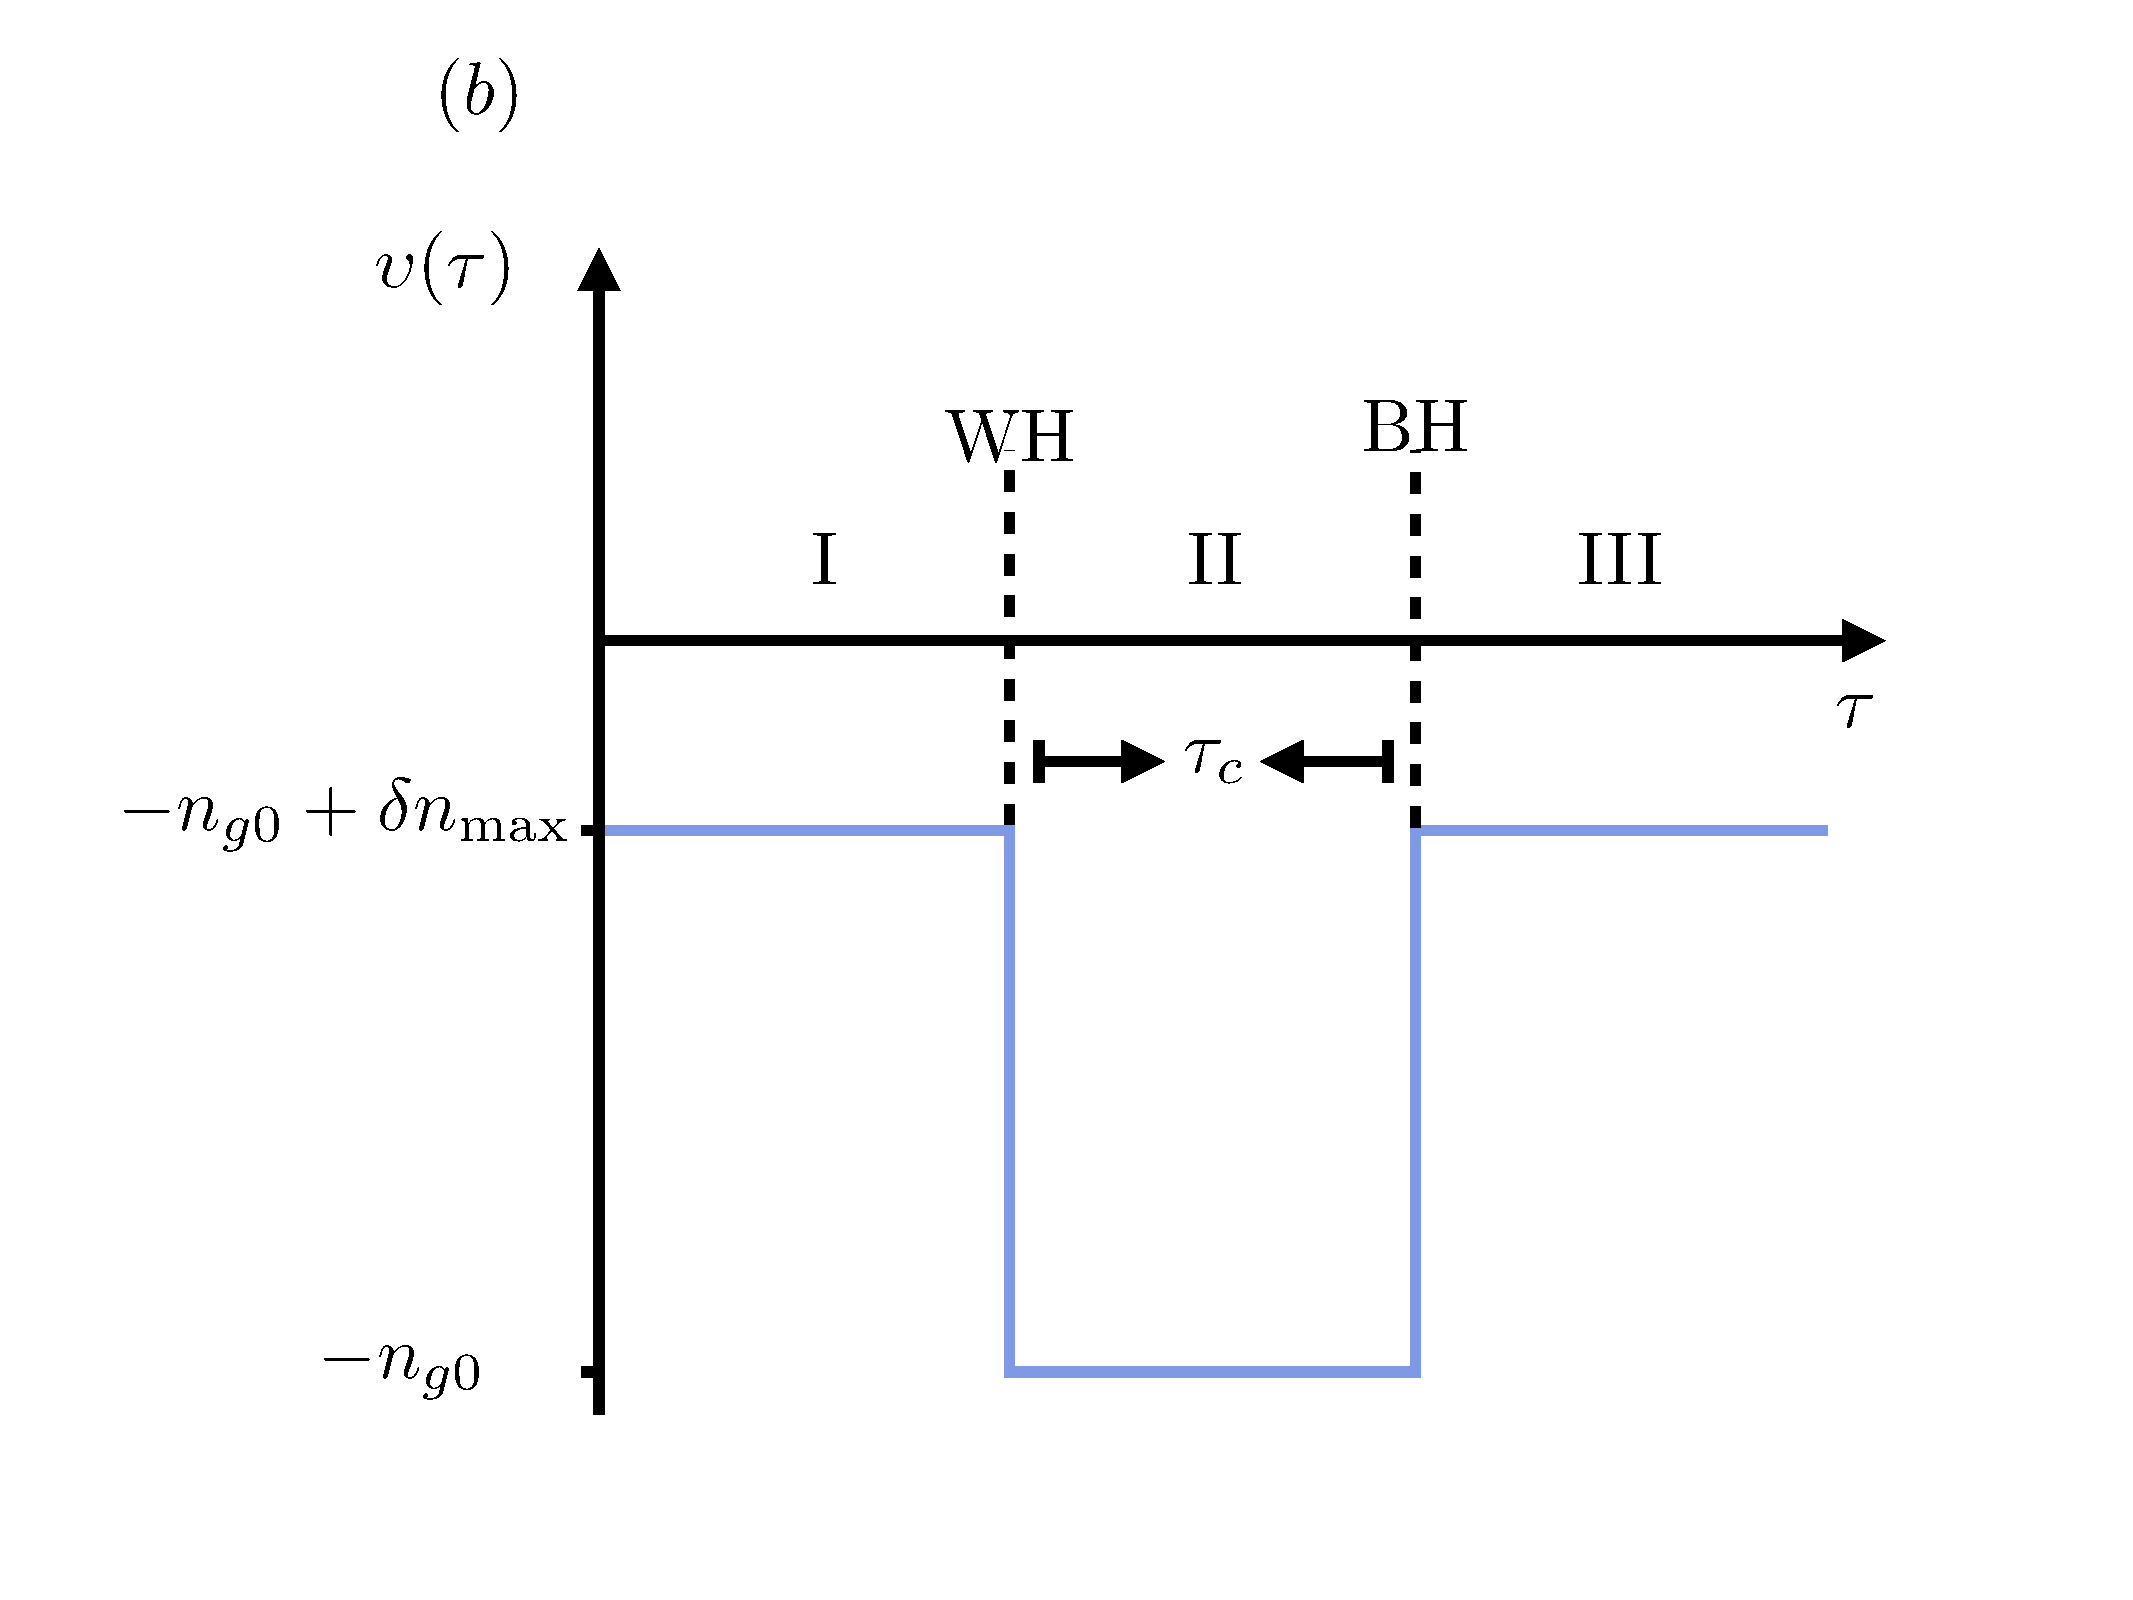
\includegraphics[height=5cm]{jdc2-2.pdf}%
   \caption{(a) Relaci\'{o}n de dispersi\'{o}n en el marco com\'{o}vil. Se encuentran cuatro modos $\omega_{\text{2u}},\omega_{\text{2v}},\omega_{\text{2ur}}$ y $\omega_{\text{2ul}}$ para la relaci\'{o}n de dispersi\'{o}n con $\delta n=0$ (l\'{i}nea verde) que define la regi\'{o}n r\'{a}pida. Para la relaci\'{o}n de dispersi\'{o}n con $\delta n=\delta n_{\text{max}}$ (l\'{i}nea morada) que define la regi\'{o}n lenta se encuentran solo dos modos $\omega_{\text{1u}}$ y $\omega_{\text{1v}}$ con $\omega'=0.294\text{PHz}$, $\Omega_0=1.861\text{PHz}$, $n_{g0}=1.488$, estos son par\'{a}metros reales para una fibra de cristal fot\'{o}nico (PFC) y $\delta n_{\text{max}}=0.1$. (b) Perfil de velocidad $\upsilon(\tau)$ que define el OBHL.} 
   \label{fig:5.1}
\end{figure}

\section{Direcci\'{o}n de viaje}\label{dirviaje}
La direcci\'{o}n de viaje para modos que son soluci\'{o}n a la relaci\'{o}n de dispersi\'{o}n en el marco de laboratorio est\'{a} dada por
\begin{align}
v_g(\omega,\delta n)=\frac{\partial\omega}{\partial \beta}=\frac{c}{\delta n+\displaystyle \sqrt{1+\frac{\omega^2}{\Omega_0^2}}\left(\frac{2\omega^2+\Omega_0^2}{\omega^2+\Omega_0^2}\right)},
\end{align}
los modos contrapropagantes (u) se mover\'{a}n con velocidad positiva, recuerde que por convenci\'{o}n el flujo con que se mueve el medio es negativo,
\begin{equation}
v_g^{\text{u}}(\omega,\delta n)=v_g(\omega,\delta n).
\end{equation}

Cuando $\delta n=\delta n_{\text{max}}$ se tienen los modos en la regi\'{o}n lenta (1u), mientras que si $\delta n=0$ se tienen los modos de la regi\'{o}n r\'{a}pida (2u). Los modos copropagantes (v), por otro lado se mueven en la misma direcci\'{o}n del fluido, por tanto su velocidad es negativa, as\'{i}

\begin{align}
v_{g}^{\text{v}}(\omega,\delta n)=-v_g(\omega,\delta n),
\end{align}
nuevamente, cuando $\delta n=\delta n_{\text{max}}$ se tienen los modos en la regi\'{o}n lenta (1v), mientras que si $\delta n=0$ se tienen los modos de la regi\'{o}n r\'{a}pida (2v). La velocidad normalizada con la velocidad de la luz $c$ para estos modos en el marco de laboratorio se muestra en la figura \ref{fig:5.2}(a). Observe que debido a que el r\'{e}gimen de dispersi\'{o}n es normal, a medida que la frecuencia aumenta la velocidad disminuye.\\

En el marco com\'{o}vil el n\'{u}mero de onda $\beta ' $ transforma como
\begin{align}
\beta'=\beta-\frac{u}{c^2}\omega,
\end{align}
por tanto 
\begin{align}
\nonumber v'_{\text{1u}}&=\frac{v_g^{\text{u}}(\omega,\delta n_{\text{max}})-u}{1-v_g^{\text{u}}(\omega,0)u/c^2}, \qquad v'_{2\text{u}}=\frac{v_g^{\text{u}}(\omega,0)-u}{1-v_g^{\text{u}}(\omega,0)u/c^2},\\
 v'_{\text{1v}}&=\frac{v_g^{\text{v}}(\omega,\delta n_{\text{max}})-u}{1-v_g^{\text{v}}(\omega,0)u/c^2}, \qquad v'_{2\text{v}}=\frac{v_g^{\text{v}}(\omega,0)-u}{1-v_g^{\text{v}}(\omega,0)u/c^2}.
\end{align}
Cada una de estas velocidades normalizadas con $c$ son mostradas en la figura \ref{fig:5.2}(b). Como es de esperar todas cumplen la regla de adici\'{o}n de velocidades de Einstein. A diferencia del caso sónico estudiado en el cap\'{i}tulo \ref{cap3}, ahora las frecuencias bajas son las que cambian de dirección, esto es debido a que en el caso sónico la dispersión era anómala para obtener un BHL, su velocidad aumenta con la frecuencia. En este caso tenemos una dispersión normal, cuya velocidad disminuye con la frecuencia. Por tanto, la región de frecuencias que cambia de dirección se invierte. La regi\'{o}n para la cual la direcci\'{o}n de los modos 2u se invierte est\'a marcada por l\'{i}neas discont\'{i}nuas verticales en la figura \ref{fig:5.2}(b) y los valores l\'{i}mites se conocen como horizontes $\pm \omega_\text{h}$.

\begin{center}
\begin{figure}[h]
\begin{minipage}[c]{0.5\textwidth}
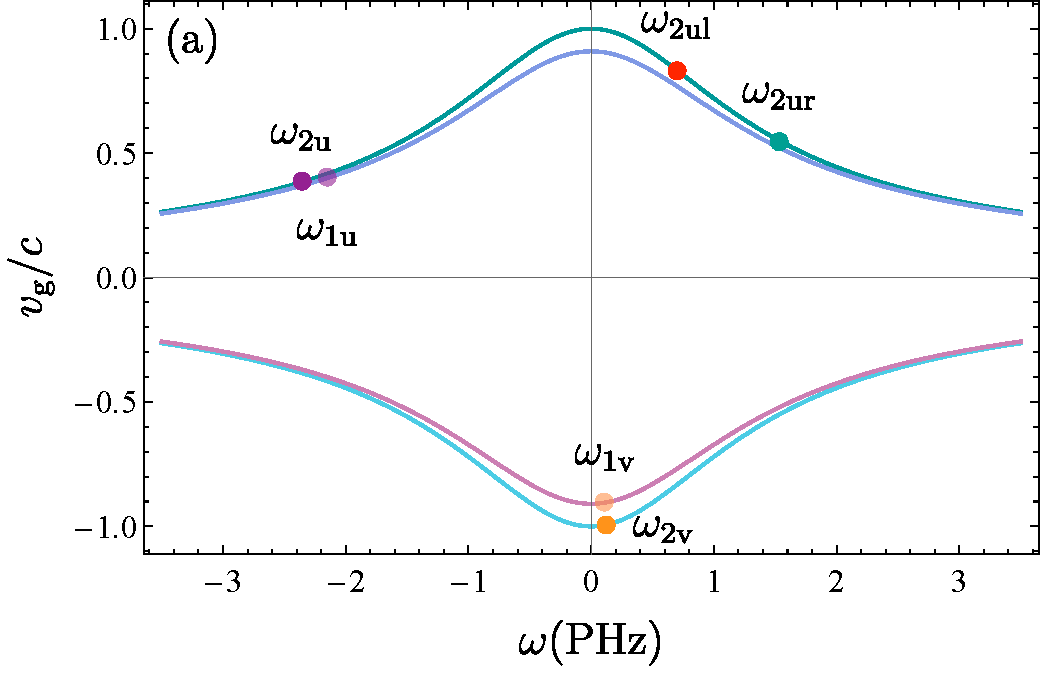
\includegraphics[width=7.5cm]{f53a.pdf}
  \end{minipage}%                       
\begin{minipage}[c]{0.5\textwidth}
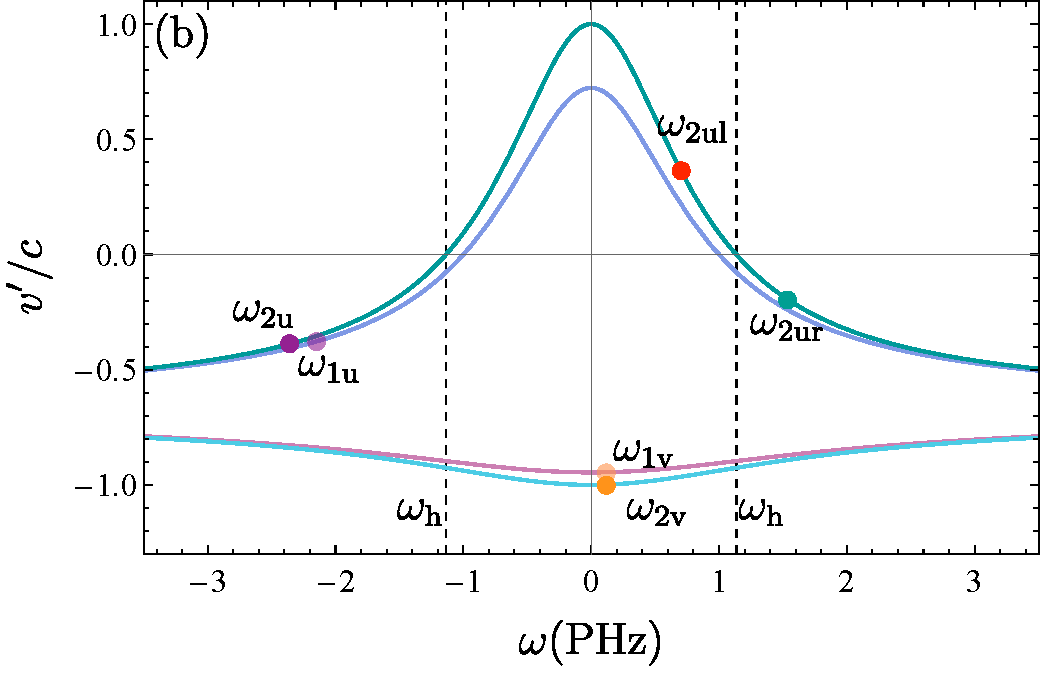
\includegraphics[width=7.5cm]{f53b.pdf}
\end{minipage}\\[2pt]                 
\caption {Velocidad de grupo para los modos $\omega$ en el marco de laboratorio (a) y en el marco com\'{o}vil (b).  Los horizontes $\pm \omega_\text{h}$ están marcados por líneas verticales entrecortadas. En ambas gr\'{a}ficas la l\'{i}nea verde indica la velocidad de modos 2u, la l\'{i}nea morada la velocidad de modos 1u, la l\'{i}nea rosa la velocidad de modos 1v y  la l\'{i}nea azul la velocidad de modos 2v. Los puntos de color indican las soluciones encontradas por el m\'{e}todo gr\'{a}fico.} 
   \label{fig:5.2}  
\end{figure}

\end{center}


\section{Horizontes}
Hemos definido el horizonte como el l\'{i}mite espacial que separa dos regiones del espacio-tiempo donde puede existir el campo o fluctuaci\'{o}n. Este l\'{i}mite f\'{a}cilmente se encuentra al igualar la velocidad de la fluctuaci\'{o}n con la velocidad del medio en movimiento. En el caso de no tener dispersi\'{o}n, como es el caso astrof\'{i}sico, el horizonte est\'{a} bien definido, es decir, cualquier frecuencia del campo siente el horizonte en el mismo lugar del espacio-tiempo, pero cuando se tiene dispersi\'{o}n como en el an\'{a}logo ac\'{u}stico u \'{o}ptico, el horizonte es difuso en el sentido de que para cada frecuencia existe un horizonte.\\

Teniendo en cuenta lo anterior definimos el horizonte $\omega_\text{h}$ como la frecuencia para la cual la velocidad con respecto a la cavidad de los modos $\omega_{\text{2u}}$ es nula, es decir, no se mueven con respecto a la cavidad. La definici\'{o}n anterior se expresa como
\begin{align}
v_{\text{2u}}(\omega)|_{\omega=\omega_{\text{h}}}=0.
\end{align}
Resolviendo la anterior ecuaci\'{o}n se encuentra como soluci\'{o}n general:
\begin{align}
\omega_{\text{h}}=\pm\frac{\Omega_0}{2\sqrt{2}}\sqrt{\upsilon^2-4\pm \upsilon\sqrt{\upsilon^2+8}},
\end{align}
donde $\upsilon=-n_{g0}+\delta n$ es el t\'{e}rmino del perfil de velocidad mostrado en la figura \ref{fig:5.1}(b). Si se cambia $\Omega_0\rightarrow k_0$ la anterior  ecuaci\'{o}n  es equivalente a la ec.(\ref{ec:horizonte}) encontrada en el caso ac\'{u}stico y la ec. ($3.4)$ de \cite{2018Bermudez}.
\section{Velocidad translum\'{i}nica}
Ahora nos planteamos si dados $\omega'$, $n_{g0}$ y $\Omega_0$ existe un velocidad $\upsilon(\tau)$ m\'{i}nima para alcanzar  el horizonte, i.e., ¿cu\'{a}l es la velocidad adimensional para que los modos $\omega_{\text{2ur}}$ y $\omega_{\text{2ul}}$ existan (son reales) y sean iguales? Llamemos a esta \textit{velocidad} \textit{translum\'{i}nica} $\upsilon_{t}=-n_{g0}+\delta n_{t}$ con $\delta n_{t}$ el cambio de \'{i}ndice de refracci\'{o}n translum\'inico. Esta cantidad puede ser encontrada anal\'{i}ticamente con una funci\'{o}n auxiliar $q(\omega',\Omega_0)$,
\begin{align}
q=270\frac{\Omega_0^2}{\omega'^2}+729\frac{\Omega_0^4}{\omega'^4}+\frac{3^{3/2}\Omega_0}{\omega'}\Bigl(27\frac{\Omega_0^2}{\omega'^2}-4\Bigr)^{3/2}-2,
\end{align}
con
\begin{align}
\delta n_{t}=\sqrt{1+\frac{\omega'^2}{3\Omega_0^2}\left(\frac{q^{1/3}}{2^{1/3}}-1\right)+\frac{2^{1/3}}{3q^{1/3}}\left(\frac{\omega'^2}{\Omega^2_0}+54\right)}.
\end{align}
Para el caso en que $\Omega_0=1.862\text{PHz}$, $\omega'=0.294\text{PHz}$, $\delta n_t=0.06<\delta n_{\text{max}}=0.1$.



\section{M\'{e}todo an\'{a}litico: OBHL con frecuencias complejas}
En esta secci\'{o}n se aplicar\'{a} la teoría de inestabilidades al láser \'{o}ptico de agujeros negros. Para esto es necesario generalizar las soluciones para frecuencias $\omega$ y $\omega'$ a complejas. Notemos que la forma can\'{o}nica de la ec. (\ref{ec:dispersion}) es
\begin{equation}
\omega^4+d\omega^3+e\omega^2+f\omega+g=0,
\end{equation}
con los siguientes coeficientes:
\begin{align}
d=0, \hspace{0.5cm} e=\Bigl(1-\upsilon^2\Bigr)\Omega_0^2, \hspace{0.5cm} f=2\upsilon\omega' \Omega_0^2, \hspace{0.5cm} g=-\omega'^2\Omega_0^2.
\end{align}
Este tipo de ecuaciones con $d=0$ pueden ser reducidas a una ecuaci\'{o}n cubica auxiliar
\begin{equation}
\omega^3+\frac{e}{2}\omega^2+\frac{e^2-4g}{16}\omega-\frac{f^2}{64}=0,
\end{equation}
a partir de sus soluciones $p_1,p_2$ y $p_3$ se obtienen la soluciones a la ecuaci\'{o}n de cuarto orden en que estamos interesados
\begin{align*}
\omega&=\sqrt{p_1}+\sqrt{p_2}+\sqrt{p_3}, \hspace{1.4cm} \omega=\sqrt{p_1}-\sqrt{p_2}-\sqrt{p_3},\\
\omega&=-\sqrt{p_1}+\sqrt{p_2}-\sqrt{p_3}, \hspace{1cm} \omega=-\sqrt{p_1}-\sqrt{p_2}+\sqrt{p_3}.
\end{align*}
\'{E}stas son las soluciones anal\'iticas para la relaci\'{o}n de dispersi\'{o}n dada en la ec. (\ref{ec:dispersion}). Aunque las soluciones explícitas son demasiado largas para escribirlas, se pueden usar para realizar cálculos analíticos con software simb\'olico. De esta manera se obtienen cuatro soluciones para cada regi\'{o}n del OBHL. El comportamiento de las cuatro soluciones complejas cuando se cambia $\upsilon(\tau)$ o el \'{i}ndice de refracci\'{o}n efectivo se muestran en la figura \ref{fig:5.4}. En esta gr\'{a}fica, se marca $v_t$, con una l\'{i}nea entrecortada indicando d\'{o}nde las soluciones $\omega_{\text{ur}}$ y $\omega_{\text{ul}}$ se hacen complejas.\\
\begin{center}
\begin{figure}
\begin{minipage}[c]{0.5\textwidth}
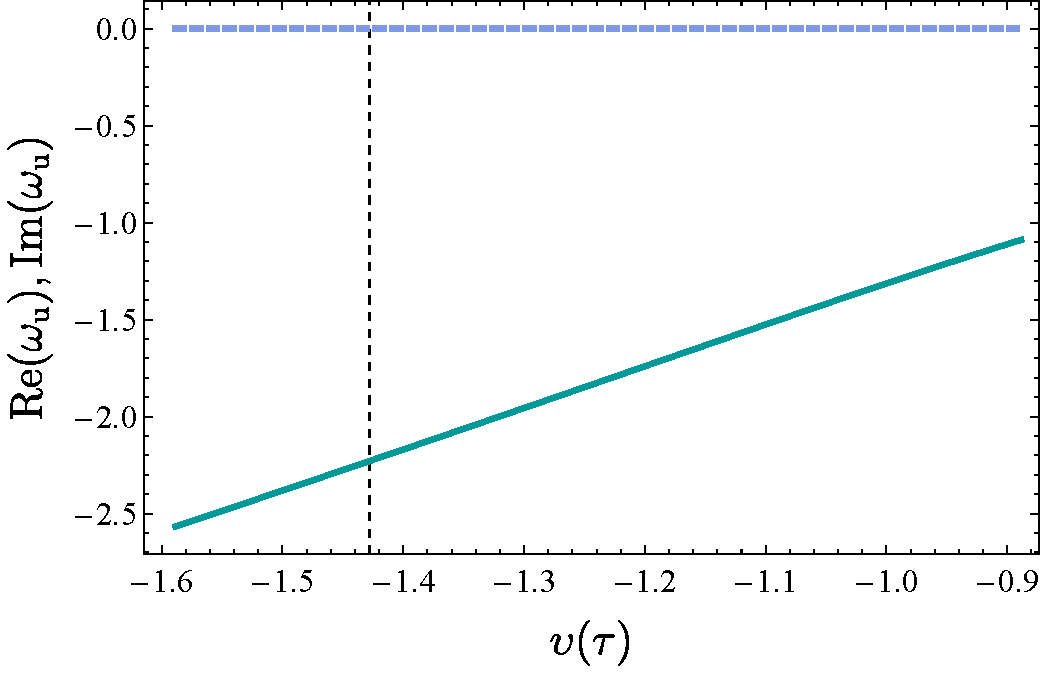
\includegraphics[width=7cm]{a1}
  \end{minipage}%                       
\begin{minipage}[c]{0.5\textwidth}
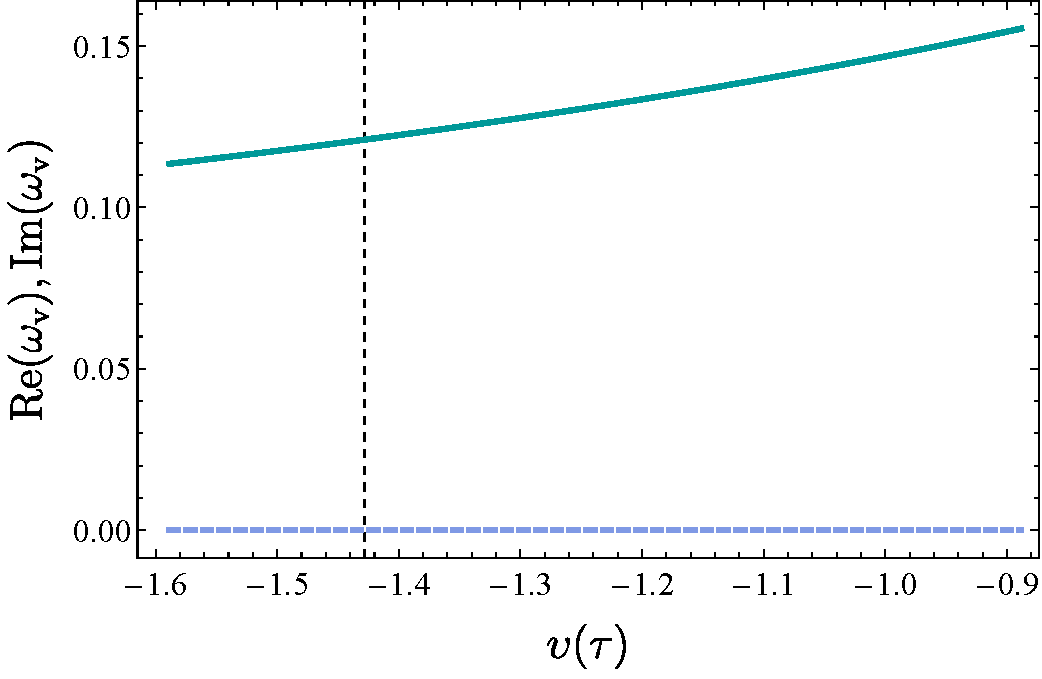
\includegraphics[width=7cm]{a2}
\end{minipage}\\[20pt]                 
\begin{minipage}[c]{0.5\textwidth}
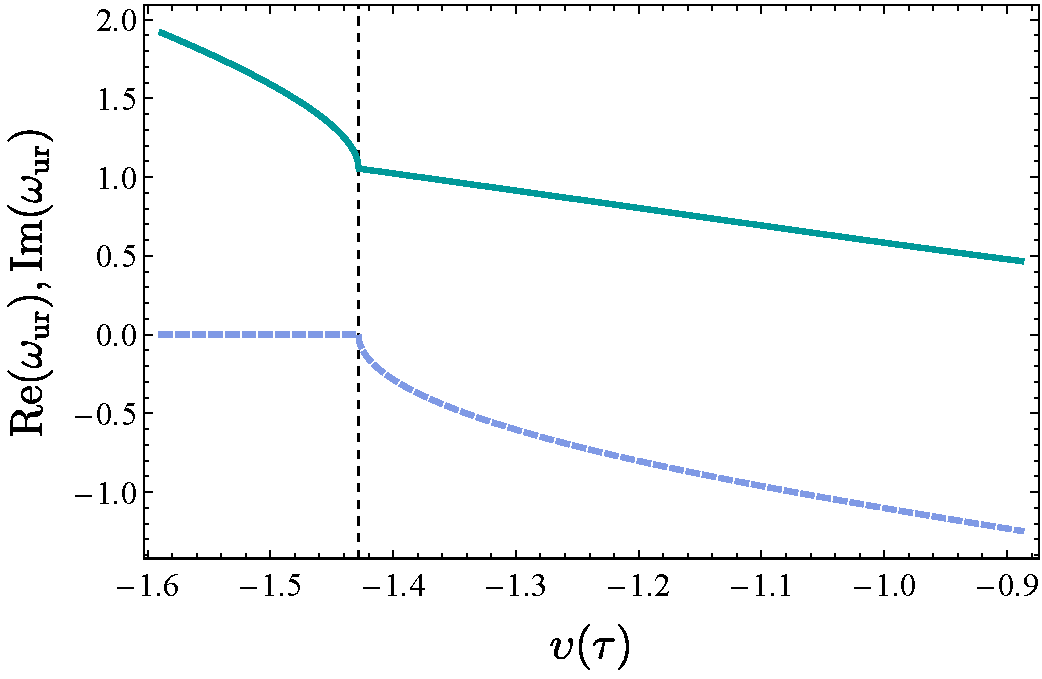
\includegraphics[width=7cm]{a3}
  \end{minipage}%
\begin{minipage}[c]{0.5\textwidth}
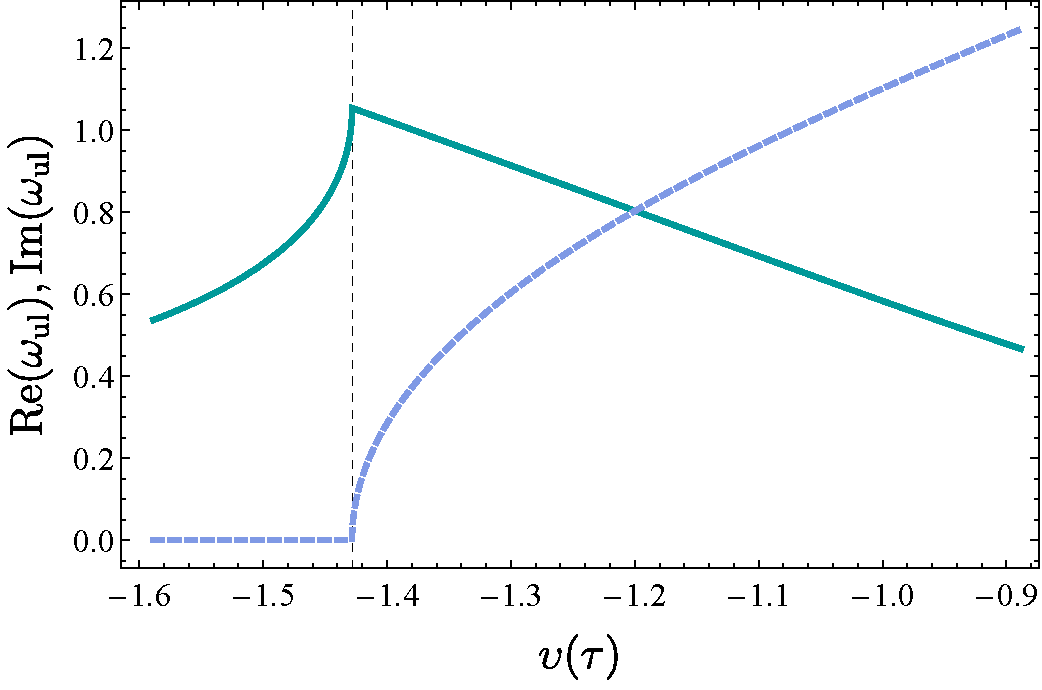
\includegraphics[width=7cm]{a4}

\end{minipage}\\[20pt] 
\caption{Las cuatro soluciones analíticas en  funci\'{o}n de la velocidad $\upsilon$, la parte real (l\'{i}nea verde continua), las parte imaginaria (l\'{i}nea morada discontinua) se muestran para $\Omega_0$ y $\omega'$ fijos. La  l\'{i}nea vertical discontinua corresponde a la velocidad translum\'{i}nica $\upsilon_t$. Podemos ver que $\omega_{\text{u}}$ y $\omega_{\text{v}}$ son reales para todas las velocidades, mientras que $\omega_{\text{ur}}$ y $\omega_{\text{ul}}$ son reales para valores de $\upsilon$ menores a $\upsilon_t$.}\label{fig:5.4}   
\end{figure}

\end{center}

Los modos o soluciones permitidas para la regi\'{o}n lenta $\upsilon_1$ y la regi\'{o}n r\'{a}pida $\upsilon_2$ que fueron analizadas en la secci\'{o}n \ref{realo} se retoman mostr\'{a}ndose en la figura \ref{fig:5.5}, que es la representaci\'{o}n en el espacio complejo para la frecuencia $\omega$. Comparando con las soluciones del método numérico, se obtienen los mismos seis resultados: cuatro para la región r\'{a}pida y  dos soluciones reales para la región lenta. Además, se obtienen dos soluciones extras que son complejas conjugadas entre sí y no aparecen en el tratamiento habitual del sistema OBHL. Estas dos soluciones adicionales en la parte lenta tienen frecuencia $\omega$ compleja, lo que genera un crecimiento o decrecimiento exponencial en los modos dependiendo de la regi\'{o}n en la que se encuentren en la configuraci\'{o}n OBHL. Tal que, si $\omega_I>0$, la soluci\'{o}n decae a la izquierda ($\tau<0)$ y si $\omega_I<0$ la soluci\'{o}n decae a la derecha ($\tau>0$)
\begin{equation}
\exp[-i\omega \tau]=\exp[-i(\omega_R+i\omega_I)\tau]=\exp[\omega_I\tau]\exp[-i\omega_R\tau].
\end{equation}

\begin{figure}\centering
	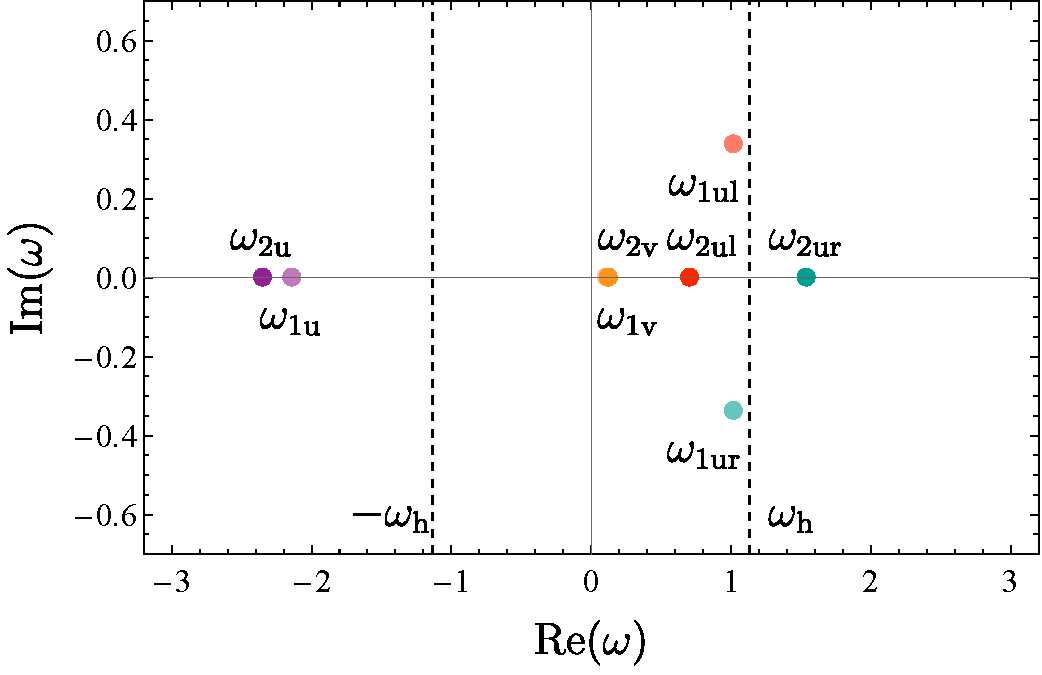
\includegraphics[width=8cm]{f55}
	\caption{Soluciones analíticas para $\upsilon_1=-n_{0g}+\delta n_{\text{max}}$ y $\upsilon_2=-n_{g0}$ en el espacio $\omega$ complejo. Se obtienen las seis soluciones reales originales más dos nuevas complejas completando las ocho soluciones al problema, cuatro pertenecen a la regi\'{o}n lenta y las otras cuatro a la regi\'{o}n rapida. Las líneas en $\omega_{\text{h}}$ ayudan a encontrar la dirección de desplazamiento de los modos: $\omega_{\text{\text{2u}}}$, $\omega_{\text{2ur}}$ y $\omega_{\text{2ul}}$.}\label{fig:5.5}
\end{figure}



\subsection{Descripci\'{o}n cualitativa y cuantitativa}
Ahora se desea encontrar las inestabilidades en el OBHL, es decir, encontrar los modos del sistema con frecuencias complejas $\omega'=\omega'_R+i\omega'_I$, donde $\omega'_I>0$, esto implica que la amplitud incrementa exponencialmente con el tiempo de propagaci\'{o}n
\begin{equation}
\exp[-i\omega' \zeta]=\exp[-i(\omega'_R+i\omega'_I)\zeta]=\exp[\omega'_I\zeta]\exp[-i\omega'_R\zeta].
\end{equation}
Al tomar la configuraci\'{o}n del OBHL como un todo se considera la situación donde los únicos modos permitidos en la regi\'{o}n lenta sean aquellos que decaen exponencialmente lejos de la cavidad. Del comportamiento de las soluciones para los modos $\omega$ mostradas en la figura \ref{fig:5.5} se observa que la soluci\'{o}n $\omega_{\text{1ur}}$ tiene parte compleja positiva indicando que decae exponencialmente a la izquierda ($\tau\rightarrow -\infty$) y $\omega_{\text{1ul}}$ (complejo conjugado de $\omega_{\text{1ur}}$) decae exponencialmente a la derecha  ($\tau \rightarrow \infty$). Este comportamiento se espera de forma cualitativa para cambios peque\~{n}os de la parte imaginaria cuando $\omega'_I>0$.\\

Lo anterior, se puede resumir de manera formal de la siguiente manera: si dividimos el campo cu\'{a}ntico $\phi$ en tres regiones I, II y III:
\begin{align}
\phi_I=\textbf{A}\cdot \exp[-i{\bm{\omega}}_1\tau],\qquad \phi_{II}=\textbf{B}\cdot \exp[-i{\bm{\omega}}_2\tau]\qquad\phi_{III}=\textbf{C}\cdot \exp[-i{\bm{\omega}}_1\tau],
\end{align}

donde
\begin{align}
\textbf{A}=(A_1,A_2,A_3,A_4),\qquad\textbf{B}=(B_1,B_2,B_3,B_4),\qquad\textbf{C}=(C_1,C_2,C_3,C_4),
\end{align}
y
\begin{align}
 \exp[-i{\omega}_1\tau]&=(\exp[-i\omega_{11}\tau],\exp[-i\omega_{12}\tau],\exp[-i\omega_{13}\tau],\exp[-i\omega_{14}\tau]),\\
 \exp[-i{\omega}_2\tau]&=(\exp[-i\omega_{21}\tau],\exp[-i\omega_{22}\tau],\exp[-i\omega_{23}\tau],\exp[-i\omega_{24}\tau]).
\end{align}
En la configuraci\'{o}n del l\'{a}ser \'{o}ptico, los modos entrantes y salientes están permitidos siempre que el campo $\phi$ sea una funci\'{o}n de cuadrado integrable, raz\'{o}n  por la cual en el parr\'{a}fo anterior se pide que sean exponenciales que decaen fuera de la cavidad. Esto significa que la configuración de OBHL es
$A_1 = A_2 = C_3 = C_4 = 0$, como se indica en la figura \ref{F56}. Los otros coeficientes se deben encontrar para definir por completo el campo cu\'{a}ntico en la configuraci\'{o}n OBHL.


\begin{figure}\centering
	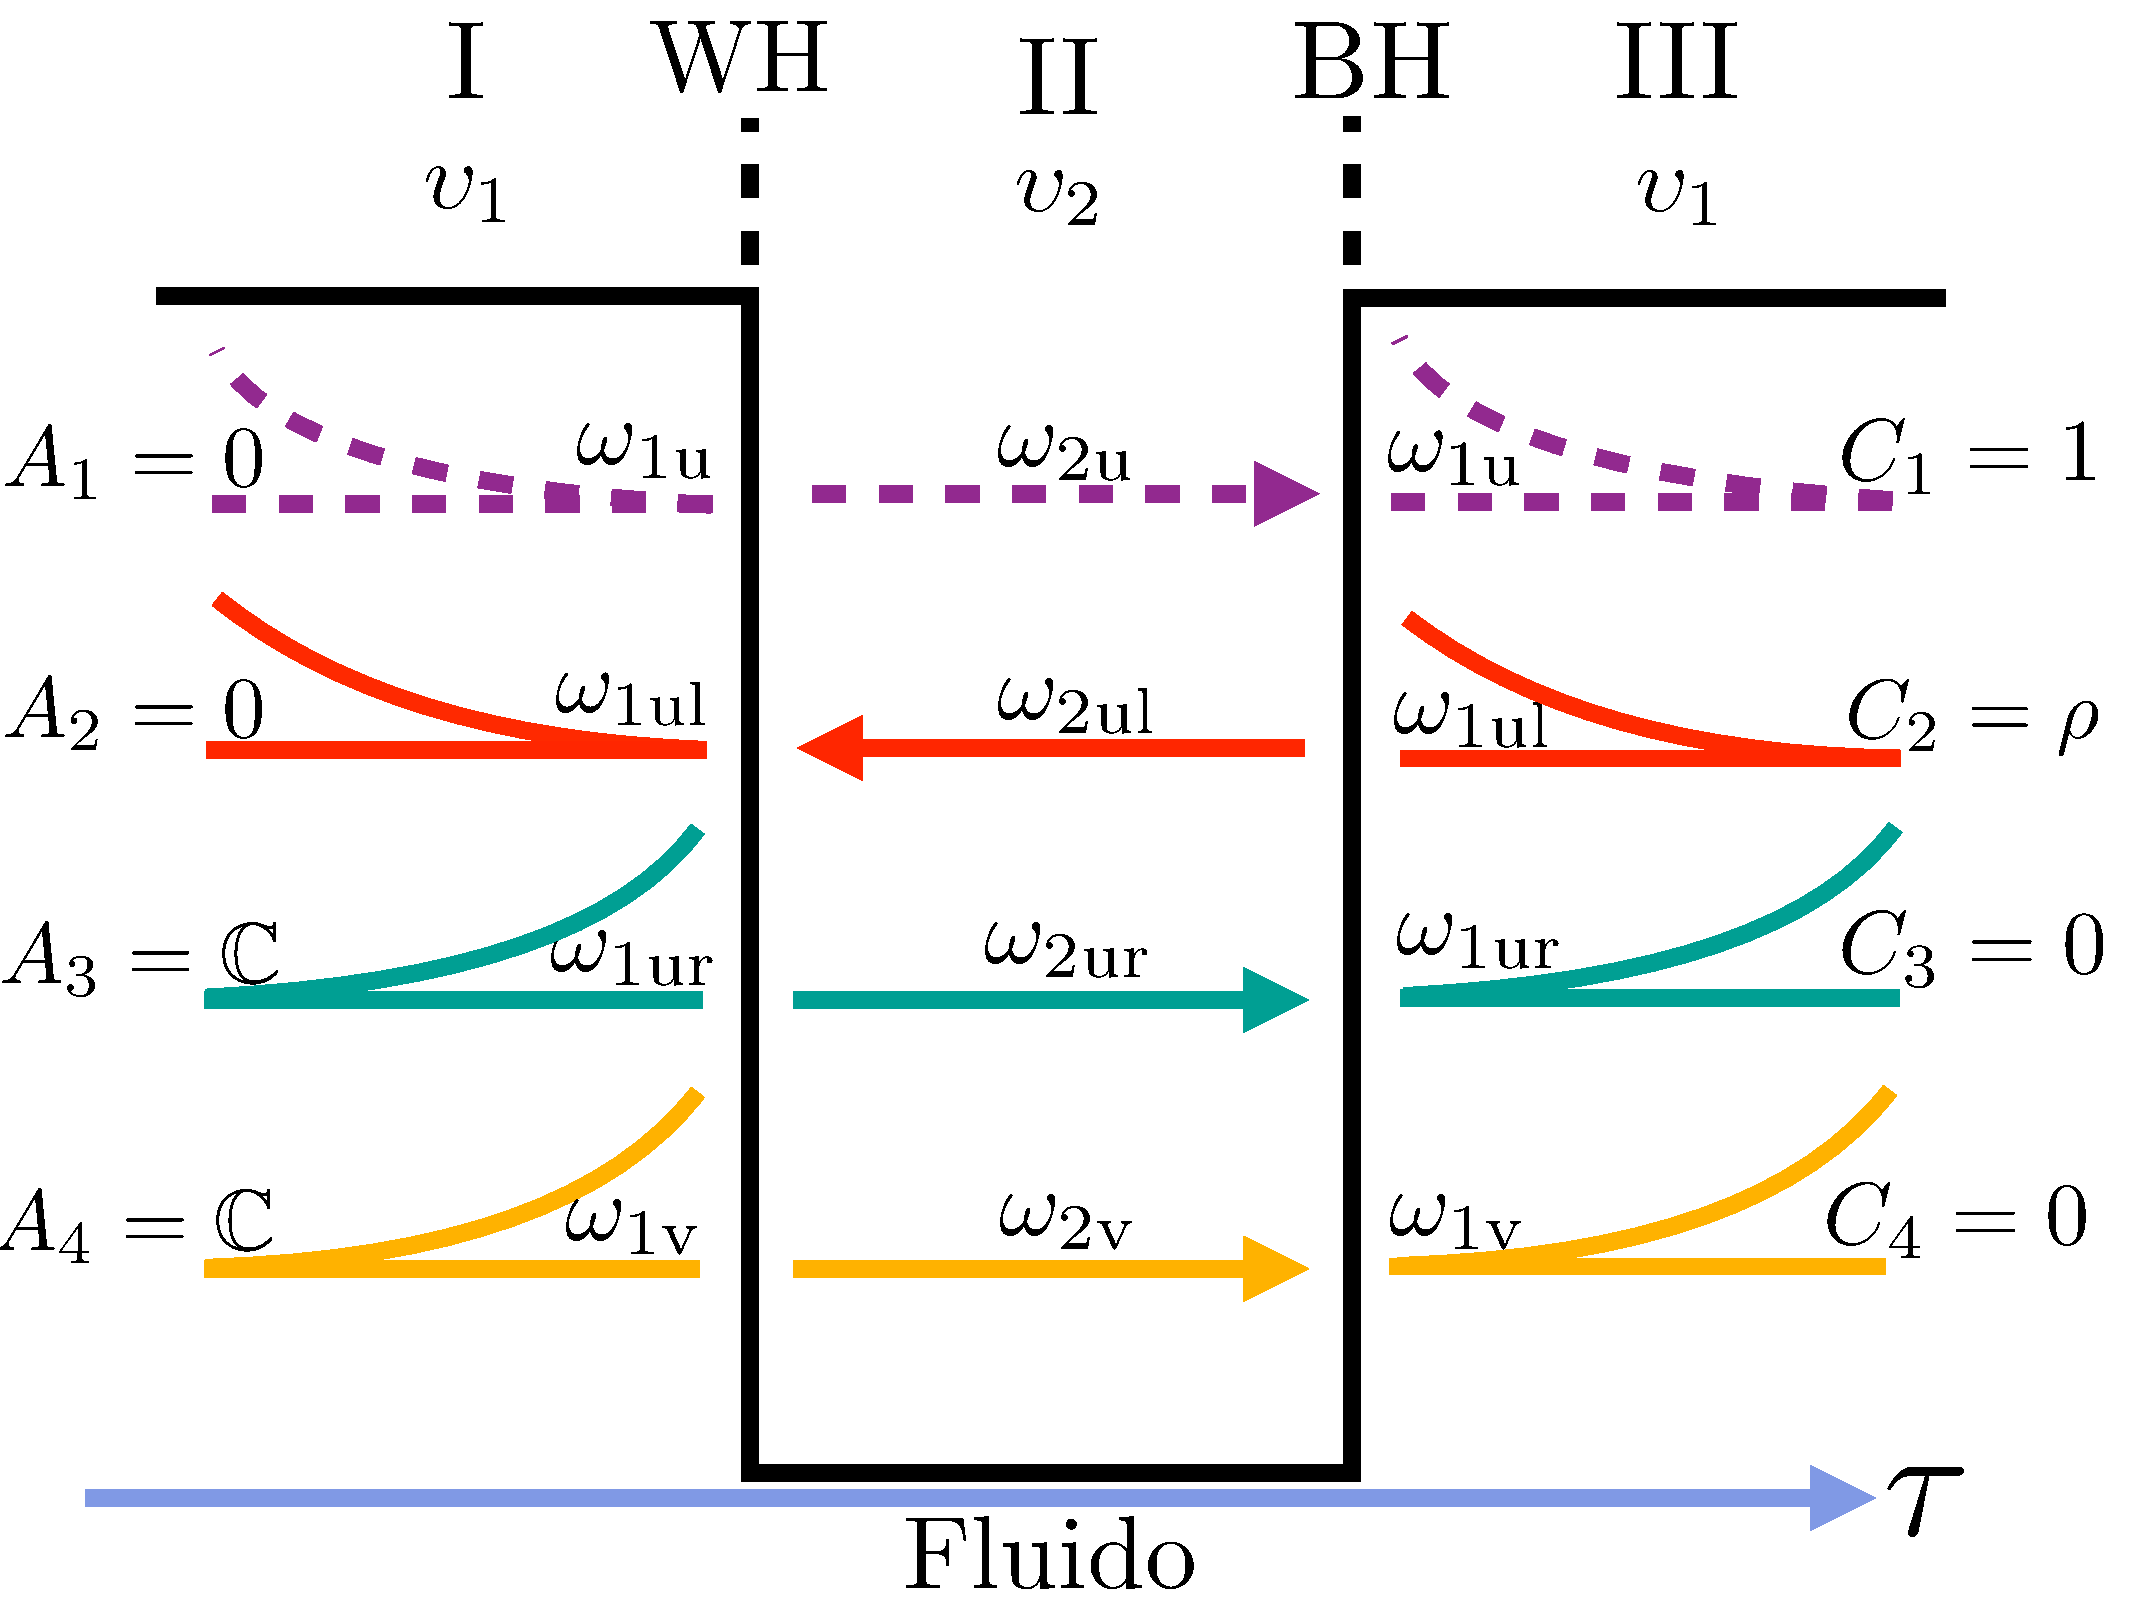
\includegraphics[height=7.5cm]{ultima}
	\caption{Diagrama de modos de una OBHL con inestabilidades en el marco com\'{o}vil, con cordenadas ($\tau,\zeta$). Los coeficientes mostrados $A_j$ y $C_j$ describen la soluci\'{o}n para que el campo $\phi$ sea una funci\'{o}n de cuadrado integrable. Recordar que en las coordenadas ($\tau, \zeta$) las direcciones de velocidades calculadas en la secci\'{o}n \ref{dirviaje} cambian de sentido debido a la transformaci\'{o}n de coordenadas dada en la ec. (\ref{trans2}). Las l\'{i}neas discontinuas indican modos con norma negativa y las continuas modos con norma positiva.}\label{F56}
\end{figure}

\subsection{Estados confinados}
Para resolver este problema se aplicar\'{a} el método de matriz de transferencia empleado en la secci\'{o}n \ref{matriztransferencia}. Se puede usar este método porque el perfil de velocidad es constante en todas las regiones excepto en las interfaces, donde se debe condicionar la continuidad del campo cuántico $\phi(\tau)$ y sus tres primeros derivadas $\phi'(\tau), \phi''(\tau),\phi'''(\tau)$ (ya que tenemos una ecuación diferencial de cuarto orden ec. (\ref{ec:dinamica})).
Para definir las matrices de transferencia o salto de la región I a la regi\'{o}n II como ($M_1$) y de la regi\'{o}n II a la regi\'{o}n III como ($M_2$) usamos las matrices auxiliares $m_1$ y $m_2$  cuyas entradas ser\'{a}n coeficientes del campo y sus derivadas ($\phi,\phi', \phi'',\phi'''$):
\begin{eqnarray*}
m_1=\begin{pmatrix}
1 & 1 & 1 & 1 \\ 
-i\omega_{11} &-i\omega_{12}  & -i\omega_{13} &-i\omega_{14} \\ 
-\omega_{11}^2 &- \omega_{12}^2 &-\omega_{13}^2  &-\omega_{14}^2 \\ 
 i\omega_{11}^3&  i\omega_{12}^3&  i\omega_{13}^2 & i\omega_{14}^3
\end{pmatrix},\quad m_2=\begin{pmatrix}
1 & 1 & 1 & 1 \\ 
-i\omega_{21} &-i\omega_{22}  & -i\omega_{23} &-i\omega_{14} \\ 
-\omega_{21}^2 &- \omega_{22}^2 &-\omega_{23}^2  &-\omega_{24}^2 \\ 
 i\omega_{21}^3&  i\omega_{22}^3&  i\omega_{23}^2 & i\omega_{24}^3
\end{pmatrix}.
\end{eqnarray*} 

El primer sub\'{i}ndice en $\omega_{ij}$ corresponde a la velocidad $\upsilon_1$ o $\upsilon_2$, el segundo especifica la soluci\'{o}n de 1-4. Es posible seleccionar cualquier orden para las soluciones de $\omega$ siempre y cuando se mantenga el orden escogido, aqu\'{i} se ha ordenado como u, ul, ur y v como se muestra en la figura \ref{F56}. Entonces las matrices de tranferencia son simplemente 
\begin{align}
M_1=m_2^{-1} m_1, \hspace{2cm}M_2=m_1^{-1} m_2=M_1^{-1}.
\end{align}
También es conveniente definir las matrices de propagación para tomar la solución entre las interfaces de la cavidad.
\'{E}stas son
\begin{align}
 P_L&=\text{diag}(\exp[i\omega_{21}\tau_c],\exp[i\omega_{22}\tau_c],\exp[i\omega_{23}\tau_c],\exp[i\omega_{24}\tau_c]),\\
P_R&=\text{diag}(\exp[-i\omega_{21}\tau_c],\exp[-i\omega_{22}\tau_c],\exp[-i\omega_{23}\tau_c],\exp[-i\omega_{24}\tau_c]).
\end{align}
Finalmente, la matriz de transferencia $(M)$ de la regi\'{o}n III a la regi\'{o}n I est\'{a} dada por

\begin{align}\label{matrizM}
M=M_1P_LM_2=m_2^{-1}m_1P_Lm_1^{-1}m_2.
\end{align}
De manera similar, para pasar de la regi\'{o}n III a la regi\'{o}n I se tiene $M^{-1}$. Usando $M$, se pueden tener los coeficientes $\textbf{A}$ en t\'{e}rminos de los $\textbf{C}$, a trav\'{e}s de
\begin{equation}
\phi_I=M\phi_{III}.
\end{equation} 
Para cada $\omega'$ existe un conjunto de cuatro n\'{u}meros de onda $\omega$ en la regi\'{o}n lenta $\bm{\omega}_1$ y otros cuatro en la regi\'{o}n r\'{a}pida $\bm{\omega}_2$.\\

Este problema se puede resolver analíticamente ya que a partir de los cuatro coeficientes $\textbf{C}$ (o $\textbf{A}$), se pueden determinar los ocho números de onda complejos correspondientes
$\bm{\omega}_1(\omega')$ y $\bm{\omega}_2(\omega')$ para cualquier frecuencia compleja y finalmente calcular los cuatro coeficientes\textbf{ A} (o \textbf{C}).\\

Con las condiciones mostradas en la figura \ref{F56} definimos un modo espontáneo del láser \'{o}ptico como un modo del OBHL donde el campo $\phi(\tau)$ es una funci\'{o}n de cuadrado integrable con frecuencia compleja y parte imaginaria positiva. La solución con un coeficiente nulo se puede encontrar analíticamente, pero con un segundo, el problema tiene que ser resuelto numéricamente. Variando los par\'{a}metros $\delta n_{\text{max}}$ y $\tau_c$ con los que se construye la cavidad se logra encontrar los modos propios $\omega'_l$ de la cavidad, aqu\'{i} el subíndice $l$ indica que es un modo del láser. En la tabla \ref{tabla:1} se muestra el \textit{n\'{u}mero de inestabilidades} ($N_{ins}$) o frecuencias complejas que se obtienen para un mismo conjunto de par\'{a}metros de la cavidad, siendo estos: $\tau_c=\{6,\ 13,\ 20\text{fs}\}$, y $\delta n_{\text{max}}=\{0.01, \ 0.05\}$. Adem\'{a}s se calcula la \textit{probabilidad de confinamiento} $\text{P}_{\text{c}}$ que indica la probabilidad de encontrar el campo $\phi$ en el interior de la cavidad y es definida como
\begin{equation}
\text{P}_{\text{c}}=\int_0^{\tau_c} d\tau \ |\phi(\tau)|^2,
\end{equation}
siendo $|\phi|^2$ normalizada a la unidad en todo el espacio. En las figuras \ref{fig:5.7B} se muestra la densidad de probabilidad $|\phi|^2$ para los modos de la cavidad expuestos en la tabla \ref{tabla:1}. Observe que $N_{ins}$ indica el n\'umero de excitaciones posibles para un estado de la cavidad caracterizado por $\tau_c$ y $\delta n_{\text{max}}$ y a su vez las posibles resonancias del modo cuando se analiza por un modelo simple (ver secci\'{o}n \ref{resonancia}). \\

Observe que para las soluciones encontradas en general $\text{P}_{\text{c}}< 100\%$, esto significa que existe una probabilidad de que el campo logre tunelar y escapar de los horizontes, un comportamiento t\'{i}pico de la radiaci\'{o}n de Hawking. Este mismo comportamiento se observa en los sistemas ac\'{u}sticos como el tratado en el cap\'{i}tulo \ref{cap3} y \cite{2018Bermudez}, y tambi\'{e}n reportados en \cite{curtis2019evanescent} y \cite{coutant2019slow}. Aunque no es posible suprimir este comportamiento que es propio de la HR, existen par\'{a}metros para la construci\'{o}n de la cavidad con los que se encuentra que $\text{P}_{\text{c}}$ es cercano al $100\%$ indicando que es posible confinar luz con luz dentro de una fibra \'{o}ptica. Lo anterior expresa a nivel cualitativo el comportamiento de una gu\'{i}a de onda temporal para pulsos \'{o}pticos expuesta en \cite{Plansinis2016}.\\

De la tabla \ref{tabla:1} y las figuras \ref{fig:5.7B} se observa que el estado base aumenta su confinamiento a medida que hacemos m\'as grande la cavidad, i.e., el incrementar $\tau_c$ y $\delta n_{\text{max}}$ incrementa $\text{P}_{\text{c}}$.\\

\begin{table}
\centering
\begin{tabular}{|c|c|c|c|c|c|}\hline
$\tau_c(\text{fs})$&$\delta n_\text{{max}}$&$N_{ins}$&$\omega_l '(\text{PHz})$& $\text{P}_{\text{c}}(\%)$&$x_f$(m)\\
\hline \hline
\multirow{2}{*}{6} & 0.01 & $1$&$0.351+i 1.64\times10^{-6}$&36&9.23\\ \cline{2-6}
& 0.05 &1&$0.333+i6.12\times 10^{-5}$& 47&0.251\\ \cline{1-6}
\multirow{3}{*}{13} & \multirow{1}{*}{0.01}& \multirow{1}{*}{1}& $0.355+i9.6\times10^{-7}$ &74&1.32\\ \cline{2-6}
 & \multirow{2}{*}{0.05}& \multirow{2}{*}{2}& $0.350+i1.45\times10^{-5}$&95&0.09\\ \cline{4-6}
&&&$0.32+i4.8\times10^{-5}$&36&0.31\\ \cline{1-6}
\multirow{5}{*}{20} & \multirow{2}{*}{0.01}& \multirow{2}{*}{2}& $0.356+i4.78\times10^{-7}$ &87&2.58\\ \cline{4-6}
&&&$0.349+i5.08\times10^{-7}$&21&2.52\\ \cline{2-6}
 & \multirow{3}{*}{0.05}& \multirow{3}{*}{3}&$0.354+i5.02\times10^{-6}$ &96&0.26\\ \cline{4-6}
&&&$0.337+i2.58\times10^{-5}$&11&0.063\\ \cline{4-6}
&&&$0.312+i1.16\times10^{-5}$&60&0.12\\ \cline{1-6}
\end{tabular}
\caption{Par\'{a}metros encontrados para las condiciones impuestas en la figura \ref{F56} para una cavidad con $\tau=\{6,\ 13, \ 20\}$fs, y $\delta n_{\text{max}}=\{0.01,\ 0.05\}$.}
\label{tabla:1}
\end{table}

\begin{figure}\centering
	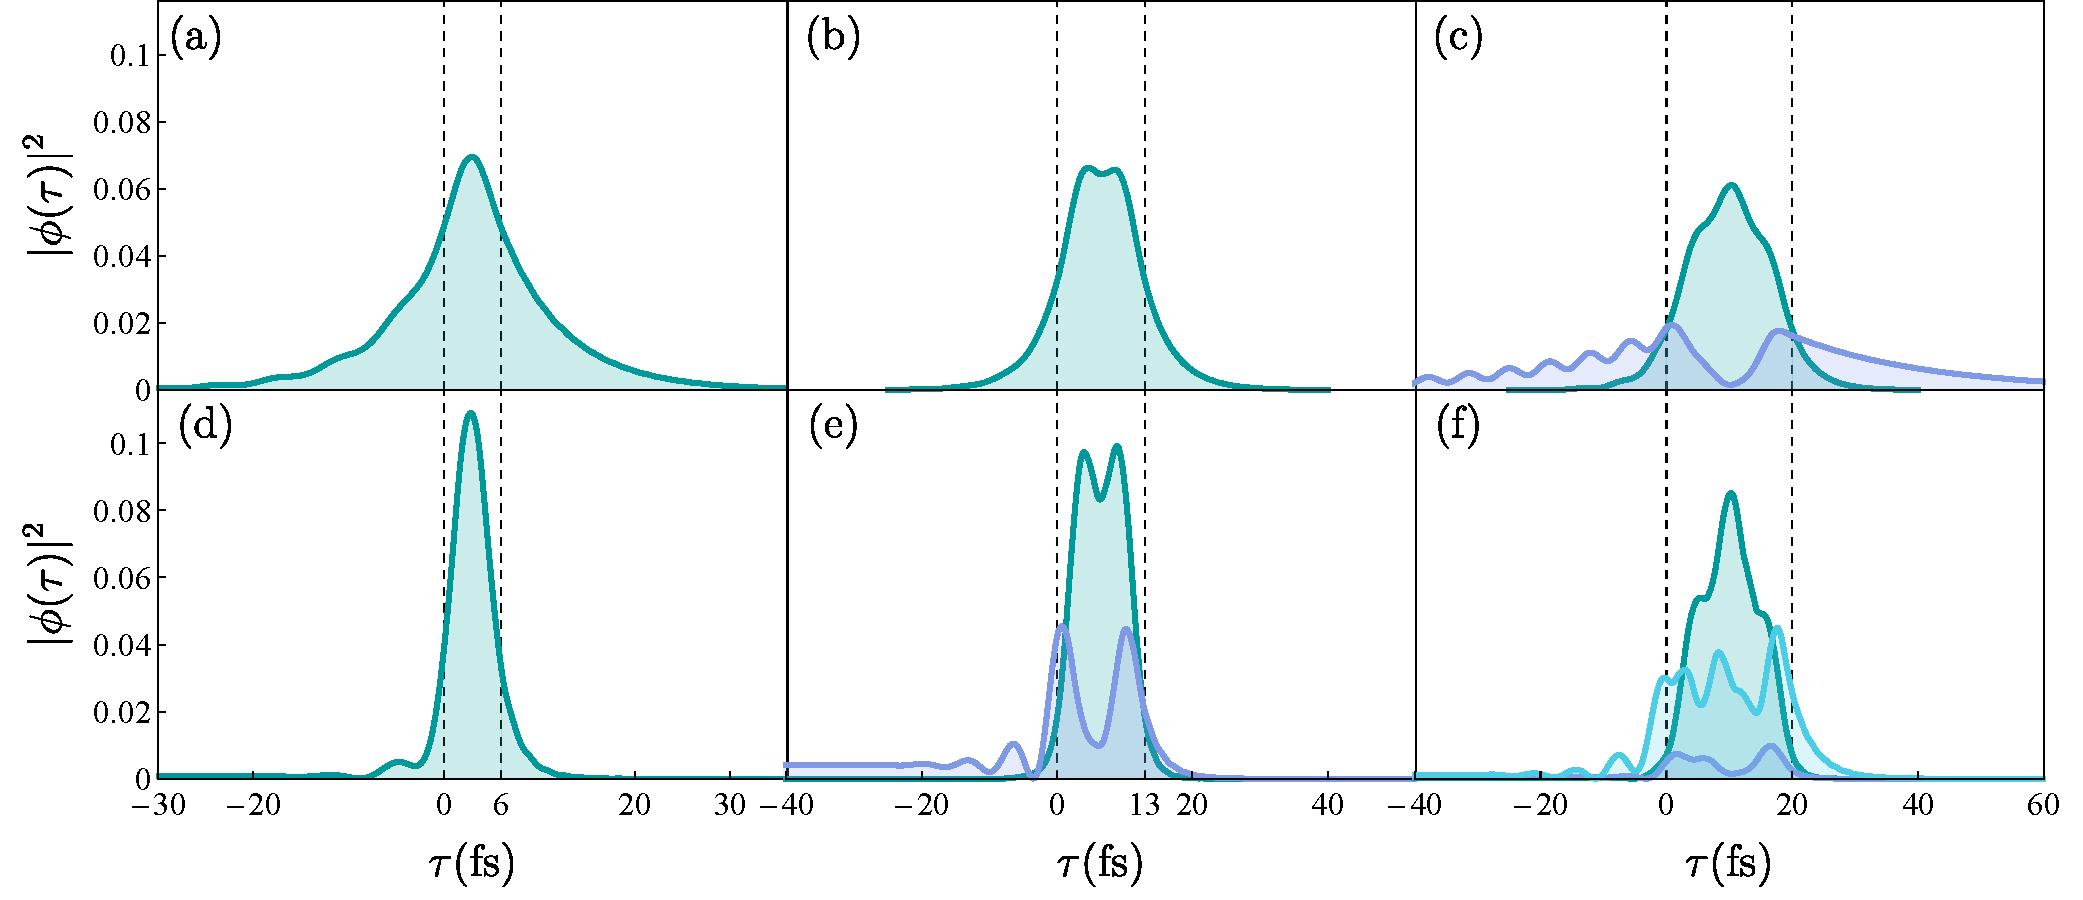
\includegraphics[width=16.cm]{lP}
	\caption{Densidad de probabilidad $|\phi
(\tau)|^2$ para modos de la cavidad encontrados por teor\'{i}a de inestabilidades y con par\'ametros dados en la tabla \ref{tabla:1}. Se grafica en verde el estado base o primera resonancia, en morado el primer estado excitado o segunda resonancia y en azul el segundo estado excitado o tercera resonancia para (a) $\tau_c=6$ y $\delta n_{\text{max}}=0.01$, (b) $\tau_c=13$ y $\delta n_{\text{max}}=0.01$,(c) $\tau_c=20$ y $\delta n_{\text{max}}=0.01$, (d) $\tau_c=6$ y $\delta n_{\text{max}}=0.05$, (e) $\tau_c=13$ y $\delta n_{\text{max}}=0.05$ y (f) $\tau_c=20$ y $\delta n_{\text{max}}=0.05$.} \label{fig:5.7B}
\end{figure}


Num\'{e}ricamente se ha encontrado un conjunto discreto de modos $\omega'_l$ para alguna condici\'{o}n $\delta n_{\text{max}}$ y $\tau_c$. En la tabla \ref{tabla:1} solo se muestran algunos casos part\'{i}culares encontrados por teor\'{i}a de inestabilidades, pero ¿es posible saber cu\'{a}ntos modos discretos o inestabilidades se pueden encontrar dados $\delta n_{\text{max}}$ y $\tau_c$? En la siguiente sección compararemos las soluciones encontradas a través de la teoría de
inestabilidades con un modelo simple, respondiendo a esta pregunta.

\begin{figure}\centering
	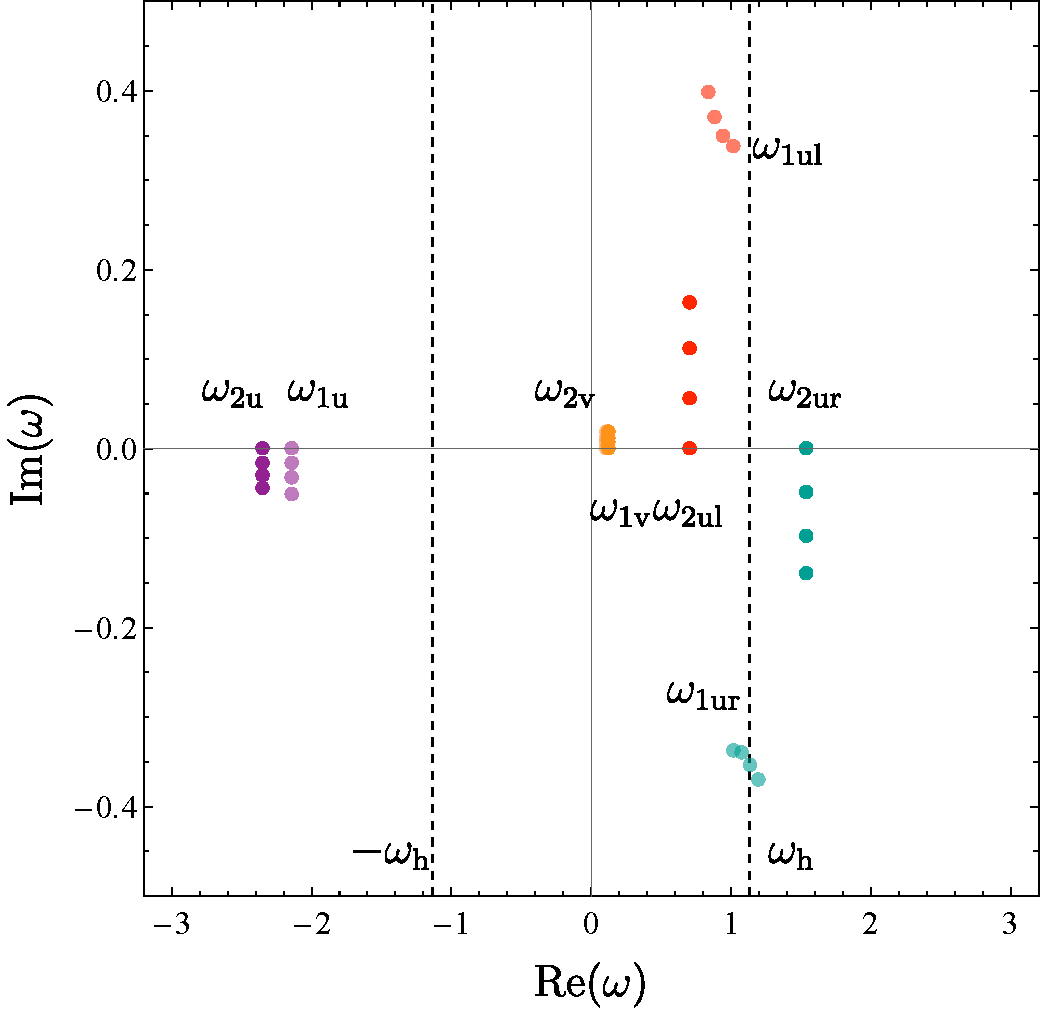
\includegraphics[width=7.cm]{f58}
	\caption{Cambio de $\bm{\omega}_1$ y $\bm{\omega}_2$ para $\text{\Re}(\omega'_l)$ fijo, e incrementando el valor de $\text{Im}(\omega')$ de $0$ a $\text{Im}(\omega'_l)$ en peque\~{n}os pasos.}\label{fig:5.8}
\end{figure}

\section{Comparaci\'{o}n del modelo de inestabilidades con el m\'{e}todo simple}
En la secci\'{o}n anterior se mostr\'{o} que por teor\'{i}a de inestabilidades se pueden encontrar los modos del OBHL. En este modelo variando las dimensiones de la cavidad $\delta n_{\text{max}}$  y $\tau_c$ se encuentra num\'{e}ricamente un conjunto discreto de soluciones o inestabilidades que son los modos del l\'{a}ser. Ahora se usar\'{a} un modelo simple para obtener una mejor imagen de la soluci\'{o}n de los modos $\omega(\omega'_l)$ con frecuencia compleja $\omega'_l=\omega'_R+i\omega'_I$, pero considerando que $\omega'_I\rightarrow 0$, que es la versi\'{o}n de una inestabilidad neutra o un modelo de onda plana con frecuencia real $\omega(\omega'_R)$.\\

Recordando la evoluci\'{o}n usual  de los modos del OBHL (ver las secci\'{o}nes \ref{BHL} y \ref{sec:real}), los modos atrapados en la cavidad son $\omega_{\text{2ur}}$ que se mueve a la derecha y $\omega_{\text{2ul}}$ que se mueve a la izquierda en el marco com\'{o}vil, permiten la creaci\'{o}n en cada ciclo de un modo que logra salir de la cavidad $\omega_{\text{1u}}$ y a su vez amplificar los modos  confinados como los que escapan de la cavidad en cada periodo. Con el modelo de onda plana se puede verificar si las soluciones de número de onda
$\omega$ siguen una condición por ciclo para una resonancia \citep{Leonhardt2007}, \citep{GaonaReyes2017}.

\subsection{Condici\'{o}n de resonancia}\label{resonancia}
\begin{center}
\begin{figure}[h]
\begin{minipage}[c]{0.5\textwidth}
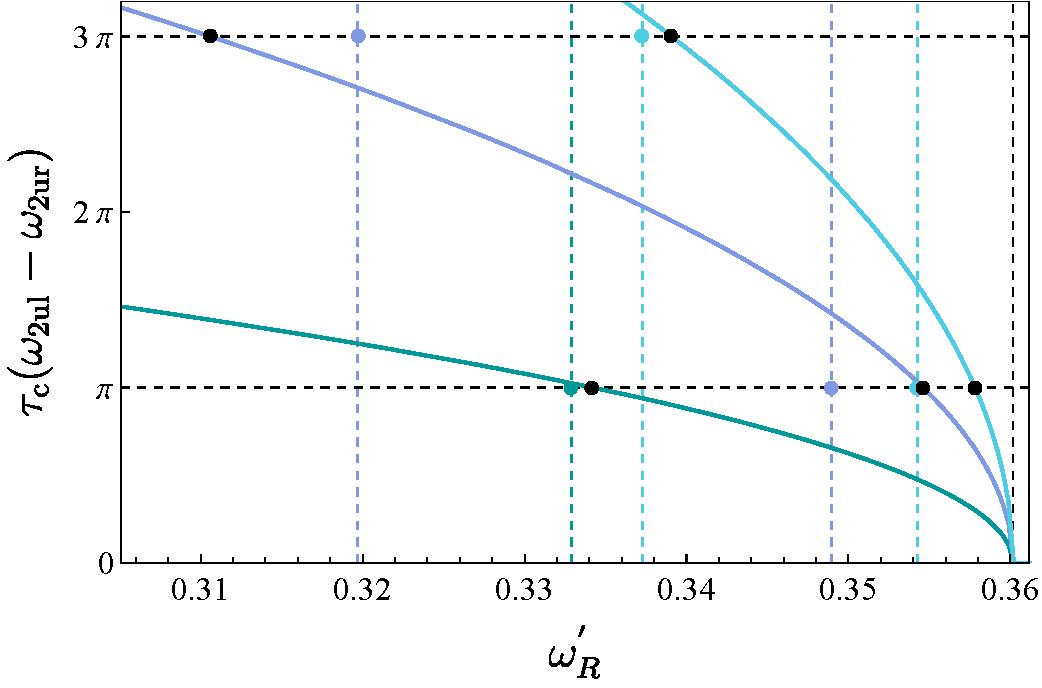
\includegraphics[width=7.5cm]{f59a.pdf}
  \end{minipage}%                       
\begin{minipage}[c]{0.5\textwidth}
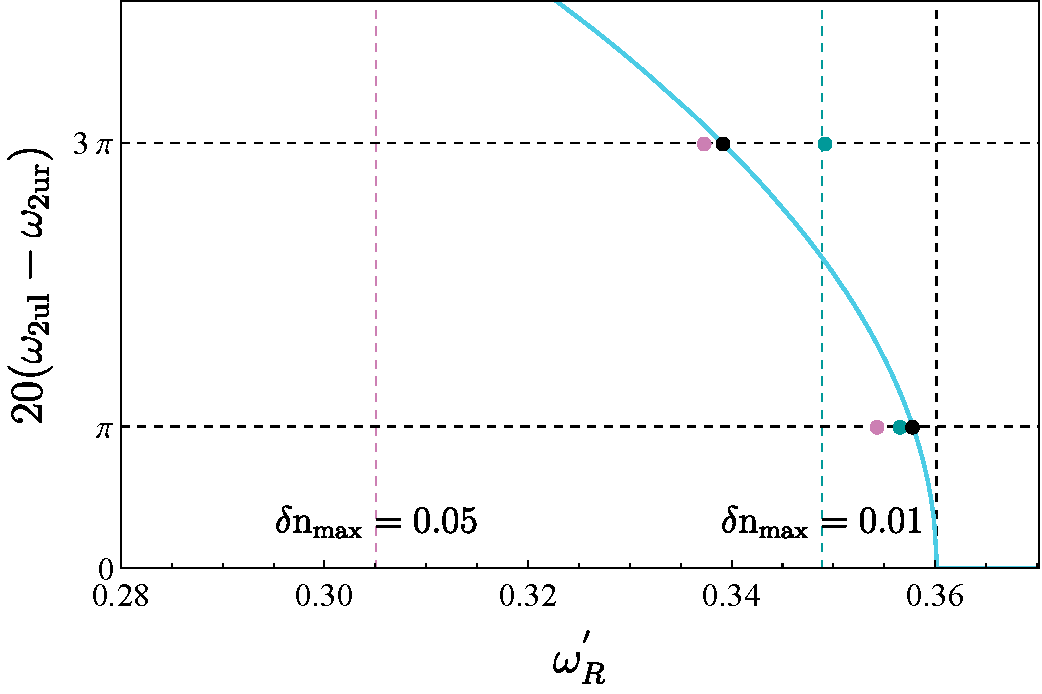
\includegraphics[width=7.5cm]{f59b.pdf}
\end{minipage}\\[2pt]                 
\caption{Diferencia de fase $\Delta \omega \tau_c .$ (a) Considerando el modelo de ondas planas cuando se fija $\delta n_{\text{max}}=0.05$  y se varia $\tau_c=\{6( \text{verde}),13(\text{morado}),20(\text{azul}) \} $fs. Las diferencias de fase de  $\pi$ y $3\pi$ predichas por el modelo cl\'{a}sico son marcadas con puntos negros. Las l\'{i}neas  verticales discontinuas marcan el valor de $\omega_R$ encontrado por teor\'{i}a de inestabilidades y su intersecci\'{o}n con la fase son los puntos de color. (b) Manteniendo fijo $\tau_c=20$ fs y variando $\delta n_{\text{max}}=\{0.05 (\text{verde}),0.01(\text{rosa})\}$. Los puntos negros son las prediciones por el modelo cl\'{a}sico, los puntos de color representan la soluci\'{o}n por el modelo de inestabilidades.}
   \label{fig:5.9}  
\end{figure}
\end{center}
\begin{figure}\centering
	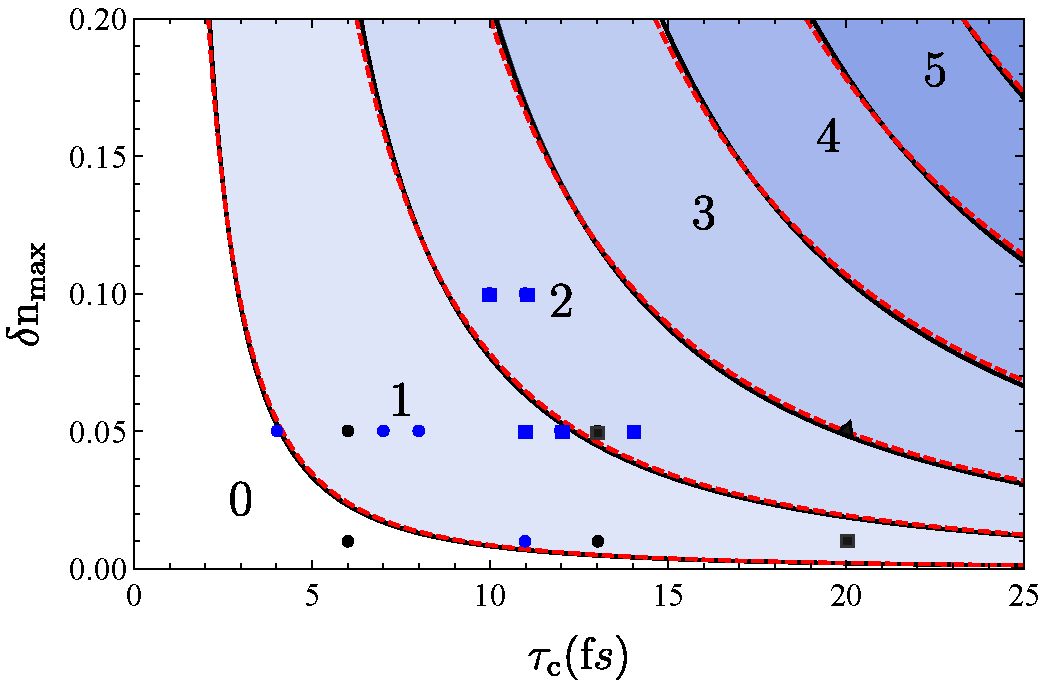
\includegraphics[width=8cm]{ultimaforma}
	\caption{N\'{u}mero de soluciones que cumplen la condici\'{o}n de resonancia en el espacio de par\'{a}metros. Dados $\delta n_{\text{max}}$ y $\tau_c$ el modelo simple indica el n\'{u}mero de resonancias. Las figuras geom\'etricas en negro son las soluciones mostradas en la tabla \ref{tabla:1}, siendo $N_{ins}=1$ para c\'irculos, $N_{ins}=2$ para rect\'angulos y $N_{ins}=3$ tri\'angulos. Las figuras geom\'etricas en azul son otras soluciones encontradas por teor\'ia de inestabilidades. Las l\'ineas discontinuas en rojo indican la cantidad de modos confinados encontrados por el modelo fenomenol\'ogico.}\label{fig:5.10}
\end{figure}

Se produce una resonancia cuando la diferencia de fase de la radiación atrapada después de un periodo de oscilaci\'{o}n es un múltiplo entero de $2\pi$. Se debe considerar que se producen dos reflexiones durante cada ciclo en
los horizontes, cada una produce un cambio de fase de $\pi/2$. Entonces, la diferencia de fase entre los modos atrapados $ \omega_{\text{2ul}}$ y $\omega_{\text{2ur}}$ debería ser
$\tau_c \Delta \omega=(2n+1)\pi$. La primera resonancia que es $\tau_c \Delta \omega=\pi$ representa en el modelo de inestabilidades el modo del l\'{a}ser en el estado base, la segunda resonacia en el modelo simple es el primer estado excitado encontrado por teor\'{i}a de inestabilidades y as\'i sucesivamente.\\

En este punto se puede analizar la condici\'{o}n de resonancia desde dos puntos de vista: manteniendo fijo $\delta n_{\text{max}}$ y variando $\tau_c$, o fijando $\tau_c$ y variando $\delta n_{\text{max}}$. Estos resultados son mostrados en las figuras \ref{fig:5.9}. Los puntos negros en las figuras \ref{fig:5.9} indican las prediciones del modelo simple, mientras los puntos de color correspondientes a la curva para la figura \ref{fig:5.9}(a) representan las soluciones encontradas por teor\'{i}a de inestabilidades cuando  $\delta n_{\text{max}}=0.05$ y $\tau_c=\{6,\ 13,\ 20\}$fs. Los puntos de igual color a las l\'{i}neas discontinuas verticales en la figura \ref{fig:5.9}(b) prepresentan las soluciones encontrada por teor\'{i}a de inestabilidades cuando variamos $\delta n_{\text{max}}$ y $\tau_c=20$fs.\\

Todas las prediciones del modelo simple son cercanas a los resultados del modelo de frecuencias complejas, los valores difieren por un error menor a $7.5\%$. Esta discrepancia podr\'{i}a explicarse debido que la condici\'{o}n de resonacia en el modelo simple no contiene informaci\'{o}n sobre $\delta n_{\text{max}}$, la \'{u}nica informaci\'{o}n necesaria para que el modelo funcione es imponer un $\delta n_{\text{max}}$ suficientemente grande tal que para un $\omega_R'$ dado se cumpla que $\delta n_{\text{max}}>\delta n_{t}$. En la figura \ref{fig:5.10} mostramos el n\'{u}mero de soluciones del modelo simple en el espacio de par\'{a}metros geom\'{e}tricos de la cavidad $(\tau_c,\delta n_{\text{max}})$. Cuando se constrasta este n\'{u}mero con el $N_{ins}$ que se encuentra en los casos part\'{i}culares mostrados en la tabla \ref{tabla:1} se observa nuevamente que el modelo simple por no ser lo suficientemente robusto no captura la soluciones para los par\'{a}metros $\tau_c=6$ y $\delta n_{\max}=0.01$ y s $\tau_c=20$ y $\delta n_{\max}=0.01$ que se encuentra por teor\'{i}a de inestabilidades.\\

Una \'ultima forma de caracterizar el n\'umero de inestabilidades o modos resonantes que puede soportar la cavidad es por medio de un modelo fenomenol\'ogico \citep{Agrawal2013}, el cual  esta dado por 
\begin{equation}\label{fenomeno}
V=\left(\frac{\omega'(\omega_h)}{2}\right)^2\tau_c^2\delta n_{\text{max}}.
\end{equation}
El par\'ametro $V$ es adimensional y depende de la geometr\'{i}a de la cavidad y el m\'{a}ximo valor de las frecuencias permitidas en el marco com\'ovil. Esta cantidad se muestra en la figura \ref{fig:5.10} con l\'ineas discontinuas rojas, mostrando evidencia que sus prediciones son una buena aproximaci\'{o}n tanto al modelo simple como al de inestabilidades. Con el modelo fenomenol\'ogico se puede predecir de forma muy sencilla cuantos modos resonantes se pueden obtener dada la geometr\'ia de la cavidad. Por ejemplo, para $0.028<V<0.253$ se obtiene un solo modo.\\

Con los resultados encontrados podemos concluir que la radiaci\'{o}n de Hawking resonante en la configuraci\'{o}n de OBHL es producto de un conjunto discreto de inestabilidades. Adem\'{a}s, dado que la $P_c<100\%$ indica que el campo puede tunelar y escapar de los horizonte, un compartamiento habitual de la radiaci\'{o}n de Hawking.

\subsection{Tiempo de propagaci\'{o}n}
Hasta el momento solo hemos verificado que los modos de la cavidad  sean funciones de cuadrado integrable en la variable $\tau$ o tiempo de retardo y que la parte real de $\omega_l'$ cumpla la condici\'{o}n de resontacia, pero ¿qu\'{e} informaci\'{o}n otorga la parte imaginaria? La parte imaginaria $\omega'_I$ de la frecuencia en el marco com\'{o}vil indica la tasa de amplificaci\'{o}n del modo de la cavidad, y a su vez permite calcular el tiempo de propagaci\'{o}n $\zeta_f$ o distancia $x_f$ que se puede mover este modo en el interior de la fibra antes de que destruya la cavidad. Para ver esto recordemos que la forma general del modo de la cavidad est\'{a} dada en la ec. (\ref{ec:ondaplana2}), que es
\begin{equation}
\phi(\tau,\zeta)=\exp[-i(\omega'_R+i\omega'_I)\zeta]\phi(\tau)=\exp(\omega_I'\zeta)\exp(-i\omega_R'\zeta)\sum_jA_j\exp(-i\omega_j\tau),
\end{equation}
tal que
\begin{equation}
 |\phi(\tau,\zeta)|^2=\exp(2\omega_{I}'\zeta)|\phi(\tau)|^2.
\end{equation}

Dado que $\omega_I>0$, la densidad de fotones $|\phi(\tau,\zeta)|^2$ (n\'{u}mero de fotones por unidad de tiempo de retardo) crecer\'{a} exponencialmente a medida que el tiempo de propagaci\'{o}n $\zeta$ avanza, por tanto, entre m\'as grande se $\omega_R$ m\'as r\'apido se amplificar el modo, pero ¿cu\'{a}nto tiempo puede amplificarse est\'e?, ¿de donde sale la energ\'{i}a para la amplificaci\'{o}n de la fluctuaci\'{o}n? El modo solo puede crecer hasta alcanzar la misma densidad de energ\'{i}a que poseen los pulso que generan la cavidad, y la energ\'{i}a que amplifica la fluctuaci\'{o}n proviene del pulso que construye los horizontes conservandose as\'{i} la energ\'{i}a del sistema .\\ 

Lo anterior nos permite construir un modelo simple para calcular el tiempo $\zeta_f$ en que existe un estado de la cavidad. La densidad de energ\'{i}a total en el sistema $\rho_{\text{S}}$ debe ser la misma en cualquier tiempo  $\zeta$. Por tanto
\begin{equation}\label{ec:49}
\rho_{\text{S}}(\zeta)=\rho_{\text{S}}(0),
\end{equation}
donde 
\begin{equation}\label{ec:50}
\rho_{\text{S}}(\zeta)=\rho^l(\zeta)+\rho^c(\zeta).
\end{equation}
El primer t\'{e}rmino a la derecha del igual es la densidad de energ\'{i}a para el modo $l$ de la cavidad y est\'a determinado por
\begin{equation}\label{ec:51}
\rho^l(\zeta)=\hbar \omega_l|\phi_{\text{max}}|^2\exp(2\omega_I'\zeta)=\rho_0^l\exp(2\omega_I'\zeta)
\end{equation}
siendo $\omega_l$ la frecuencia en el marco de laboratorio para el modo con amplitud m\'{a}xima $|\phi_{\text{max}}|^2$ que est\'a en el interior de la cavidad. El segundo t\'{e}rmino es la densidad de energ\'{i}a de los pulsos que construyen la cavidad y es
\begin{equation}\label{ec:52}
\rho_c(\zeta) =\rho_0^c\exp(-2\omega_{I}'\zeta),
\end{equation}
donde $\rho_0^c$ es la densidad de energ\'{i}a inicial de la cavidad que se va disipando a la misma tasa en que crece la energ\'{i}a de la fluctuaci\'{o}n. Para encontrar la densidad de energ\'{i}a inicial de los pulsos que construyen la cavidad recordemos de la ec. (\ref{n2}) que el $\delta n_{\text{max}}$ esta relacionado con la intensidad del pulso, por tanto
\begin{equation}
I=\frac{\delta n_{\text{max}}}{n_2},
\end{equation}
con lo cual
\begin{equation}
\rho_0^c=\frac{\delta n_{\text{max}}}{n_2}A,
\end{equation}\label{ec:53}
donde $n_2$ es el coeficiente de \'{i}ndice de refracci\'{o}n no lineal y $A$ es el \'{a}rea de la secci\'{o}n transversal de la fibra \'{o}ptica en la que se propaga el pulso. Remplazando la ec. (\ref{ec:53}) en la ec. (\ref{ec:52}) y  ec. (\ref{ec:51}) y realizando un poco de \'{a}lgebra se encuentra que
\begin{equation}
\zeta_f=\frac{1}{2\omega'_{I}}\ln\left(\frac{\rho_0^c}{\rho_0^l}\right),
\end{equation}
es el tiempo m\'{a}ximo de propagaci\'{o}n o de la ec. (\ref{trans2}) la distancia $x_f=u\zeta_f$ que puede recorrer un modo de la cavidad al propagarse en el interior de la fibra \'{o}ptica.  Para darnos una idea del orden de magnitud de la distancia $x_f$ hicimos uso de los par\'{a}metros de una PFC con $n_2=2.2\times10^{-20}\text{m}^2/\text{W}$ \citep{Agrawal2013} y $A=7.84\times10^{-14} \text{m}^2$ \citep{Bermudez2016jp}, adem\'{a}s los pulsos que crean la cavidad se propagan dentro de la fibra con una velocidad de grupo $u=0.2014\mu \text{m}/\text{fs}$. En la \'{u}ltima columna de la tabla \ref{tabla:1} se reportan las distancias de propagaci\'{o}n siendo \'{e}stas del orden de metros para cada uno de los estados encontrados.
\\